\documentclass[11pt,letterpaper]{article}

% --- Paquetes Principales ---
\usepackage[utf8]{inputenc}
\usepackage[spanish,es-nodecimaldot]{babel}
\usepackage[margin=2.5cm]{geometry}
\usepackage{amsmath,amssymb}
\usepackage{graphicx}
\usepackage{booktabs}
\usepackage{hyperref}
\usepackage{microtype}
\usepackage{xcolor}
\usepackage{caption}
\usepackage{subcaption}
\usepackage{float}
\usepackage[T1]{fontenc}
\usepackage{fancyhdr}
\setlength{\emergencystretch}{2em}

% --- Configuracion de Hipervinculos ---
\hypersetup{
    colorlinks=true,
    linkcolor=blue!70!black,
    citecolor=blue!70!black,
    urlcolor=blue!70!black
}

% --- Configuracion de Encabezados y Pies de Pagina (fancyhdr) ---
\pagestyle{fancy}
\fancyhf{}
\fancyhead[L]{\small\textsl{Boletín 01: Búsqueda en Secuencias y Colas de Prioridad}}
\fancyhead[R]{\small\textsl{Bryan Aguirre F. --- Mat. 2024443402}}
\fancyfoot[C]{\thepage}
\renewcommand{\headrulewidth}{0.4pt}
\renewcommand{\footrulewidth}{0pt}

\begin{document}
\hypersetup{pageanchor=false}

\begin{titlepage}
    \centering
    
\includegraphics[width=0.42\textwidth]{logo_udec.png}\\[1.0cm]
    
    {\scshape\Large Universidad de Concepción \par}
    \vspace{0.25cm}
    {\scshape\large Facultad de Ingeniería \par}
    {\scshape\normalsize Departamento de Ingeniería Informática y Ciencias de la Computación \par}
    \vspace{1.2cm}
    
    {\Large\textbf{Estructuras de Datos y Algoritmos Avanzados (2026-2)}\par}
    \vspace{0.6cm}
    \rule{\linewidth}{0.6mm} \\[0.4cm]
    {\huge\bfseries Boletín 01: Búsqueda en Secuencias y Colas de Prioridad \par}
    \vspace{0.3cm}
    {\large\textit{Análisis Teórico, Implementación en C++20 y Validación Experimental}\par}
    \rule{\linewidth}{0.6mm} \\[1.4cm]
    
    \begin{minipage}[t]{0.48\textwidth}
        \begin{flushleft} \large
            \textbf{Autor:}\\
            Bryan Eliseo Aguirre Fuentes\\[0.15cm]
            \textbf{Matrícula:}\\
            2024443402
        \end{flushleft}
    \end{minipage}
    \hfill
    \begin{minipage}[t]{0.48\textwidth}
        \begin{flushright} \large
            \textbf{Profesor:}\\
            Dr. José Fuentes\\[0.15cm]
            \textbf{Ayudante:}\\
            Leonardo Lovera
        \end{flushright}
    \end{minipage}
    
    \vfill
    {\large Concepción, Chile\\ \today \par}
\end{titlepage}
\hypersetup{pageanchor=true}

% =========================================================================
% ÍNDICE DE CONTENIDOS
% =========================================================================
\pagenumbering{roman}
\pagestyle{plain}
\tableofcontents
\newpage

\pagenumbering{arabic}
\pagestyle{fancy}

\section{Resumen}

\subsection{Propósito y alcance del estudio}
En este trabajo se presenta un estudio teórico y experimental comparativo sobre algoritmos fundamentales de búsqueda en secuencias y estructuras de datos para colas de prioridad. Se analizan e implementan en C++20 las búsquedas Secuencial, Binaria y Galopante, contrastando cada implementación propia frente a las utilidades optimizadas de la biblioteca estándar de C++ (STL). Asimismo, se evalúa el desempeño de las colas de prioridad, comparando el Binary Heap implementado de forma implícita sobre memoria contigua con el Binomial Heap estructurado como un bosque dinámico de punteros, a través de sus cinco operaciones: construcción, consulta de extremo, inserción, extracción y fusión.

Los experimentos empíricos se diseñaron aislando tanto el tamaño de la secuencia como la posición relativa del objetivo, empleando cronometraje de precisión a lo largo de 128 repeticiones para garantizar significancia estadística. Los resultados validan las cotas asintóticas teóricas y revelan fenómenos físicos subyacentes, tales como la saturación del bus de memoria y el impacto de la localidad espacial en la memoria caché.

\subsection{Estructuras y algoritmos}

A continuación, se describen los algoritmos de búsqueda y las estructuras de datos considerados en este trabajo:

\begin{enumerate}
    \item \textbf{Sequential Search:} Recorre secuencialmente los elementos de una secuencia hasta encontrar el objetivo o alcanzar el final.
    \item \textbf{Binary Search:} Busca un elemento en una secuencia ordenada, reduciendo a la mitad el intervalo de búsqueda en cada iteración.
    \item \textbf{Galloping Search:} Busca un elemento en una secuencia ordenada mediante saltos crecientes, generalmente de tamaño exponencial, y luego acota la búsqueda con búsqueda binaria.
    \item \textbf{Binary Heap:} Cola de prioridad implementada como un árbol binario casi completo que satisface la propiedad de heap y suele almacenarse en un arreglo.
    \item \textbf{Binomial Heap:} Cola de prioridad formada por un bosque de árboles binomiales que satisfacen la propiedad de heap y permiten fusionar dos heaps eficientemente.
\end{enumerate}

\newpage

\section{Análisis Teórico}
En esta sección se fundamentan matemáticamente los algoritmos y estructuras de datos estudiados, analizando sus complejidades asintóticas temporales en el mejor, peor y caso promedio, así como sus requerimientos espaciales y el impacto de su disposición física en memoria.


\subsection{Algoritmos de Búsqueda en Secuencias}
Los algoritmos de búsqueda tienen como objetivo determinar la presencia y posición de una clave objetivo $x$ dentro de una secuencia de $n$ elementos $A = \langle a_0, a_1, \dots, a_{n-1} \rangle$.

\begin{enumerate}
    \item \textbf{Búsqueda Secuencial (\textit{Sequential Search}):} 
    Inspecciona los elementos de forma consecutiva desde el índice $0$ hasta encontrar el objetivo o agotar el arreglo. No impone precondición de orden sobre la secuencia.
    \begin{itemize}
        \item \textbf{Mejor caso:} $\mathcal{O}(1)$, cuando el elemento reside en la primera posición ($a_0 = x$).
        \item \textbf{Peor caso:} $\mathcal{O}(n)$. El costo de una búsqueda exitosa
        depende de la posición de la primera coincidencia: si esta ocupa
        la posición $k$, contada desde 1, se realizan $k$ comparaciones
        de igualdad y el costo temporal es $\mathcal{O}(k)$. El peor caso se alcanza
        cuando $k=n$ o cuando el objetivo no pertenece al arreglo, pues
        ambas situaciones requieren examinar los $n$ elementos.
        En una implementación iterativa convencional, la búsqueda
        no exitosa realiza $n$ comparaciones de igualdad y $n+1$
        evaluaciones de la condición de continuación del ciclo.
         \item \textbf{Caso promedio:} $\mathcal{O}(n)$, condicionado a una búsqueda exitosa y suponiendo que el índice de la primera coincidencia se distribuye uniformemente entre las $n$ posiciones. Bajo este modelo, el número esperado de comparaciones de igualdad es
    \[
        \mathbb{E}[C \mid x \in A]
        = \frac{1}{n}\sum_{k=0}^{n-1}(k+1)
        = \frac{n+1}{2}.
    \]
        \item \textbf{Complejidad espacial:} $\mathcal{O}(1)$ de memoria auxiliar, operando \textit{in-place}.
    \end{itemize}

    
    \item \textbf{Búsqueda Binaria (\textit{Binary Search}):}
    Aplica el paradigma de \textit{divide y vencerás} sobre una secuencia previamente ordenada ($a_0 \le a_1 \le \dots \le a_{n-1}$). Compara el elemento central $a_{\text{mid}}$ con el objetivo $x$; si no hay coincidencia, descarta la mitad del espacio de búsqueda de forma iterativa.
    \begin{itemize}
        \item \textbf{Mejor caso:} $\mathcal{O}(1)$. En la búsqueda binaria con salida temprana (\textit{early exit}), cuando el elemento buscado se encuentra justo en la posición central solo requiere de un acceso, volviendo la complejidad temporal constante. En cambio, en una implementación convencional como \texttt{std::lower\_bound}, se continúa delimitando la primera posición cuyo valor no es menor que el objetivo, por lo que su complejidad es siempre $\mathcal{O}(\log n)$.
        \item \textbf{Peor y caso promedio:} $\mathcal{O}(\log n)$. En cada iteración, la búsqueda binaria reduce el tamaño del intervalo
        activo a lo sumo a la mitad. Por tanto, para un arreglo de $n \geq 1$
        elementos, tras $k$ iteraciones quedan como máximo $n/2^k$ elementos.
        Para reducir el intervalo a lo sumo a un elemento, basta con que
        \[
            \frac{n}{2^k} \leq 1
            \iff n \leq 2^k
            \iff k \geq \log_2 n.
        \]
        En consecuencia, a lo sumo $\lceil \log_2 n \rceil$ reducciones y una
        comprobación final bastan para completar la búsqueda. Bajo el supuesto
        de que cada iteración tiene costo constante, la complejidad temporal
        en el peor caso es $\mathcal{O}(\log n)$.
        \item \textbf{Complejidad espacial:} $\mathcal{O}(1)$ en la implementación iterativa, puesto que opera directamente sobre el arreglo y mantiene una cantidad constante de variables auxiliares, independiente del tamaño de la entrada.
    \end{itemize}

    \item \textbf{Búsqueda Galopante (\textit{Galloping Search}):}
    Propuesta por Bentley y Yao (también conocida como búsqueda exponencial), está diseñada para secuencias ordenadas de tamaño no acotado o donde la clave objetivo reside en un índice $k \ll n$. Opera en dos fases secuenciales:
    \begin{enumerate}
        \item \textit{Fase de Galope:} Compara $x$ sucesivamente con los índices exponenciales $2^0, 2^1, \dots, 2^i$ hasta hallar una cota superior tal que $a_{2^i} \ge x$ o $2^i \ge n$, requiriendo a lo sumo $\lfloor \log_2 k \rfloor + 1$ comparaciones.
        \item \textit{Fase Binaria:} Aplica búsqueda binaria sobre el subrango acotado $[2^{i-1}, \min(2^i, n-1)]$, cuya longitud no supera $k$, tomando $\mathcal{O}(\log k)$ comparaciones adicionales.

        La complejidad temporal global es $\mathcal{O}(\log k)$, superando asintóticamente a la búsqueda binaria $\mathcal{O}(\log n)$ cuando el objetivo se encuentra en los percentiles iniciales ($k \ll n$). En el peor escenario ($k \approx n$), su costo se acota por $\mathcal{O}(\log n)$.
        
    \end{enumerate}

    \begin{itemize}
        \item \textbf{Mejor caso:} $\mathcal{O}(1)$, cuando el objetivo se encuentra en la primera posición examinada, de modo que la búsqueda concluye tras una cantidad constante de comparaciones.
        
        \item \textbf{Peor caso:} $\mathcal{O}(\log n)$, cuando es necesario extender los saltos hasta las proximidades del final del arreglo y efectuar posteriormente la búsqueda binaria en el intervalo delimitado.

        \item \textbf{Caso promedio:} $\mathcal{O}(\log n)$, suponiendo búsquedas exitosas sobre elementos distintos y una distribución uniforme del objetivo entre las posiciones del arreglo. Aunque una búsqueda en la posición $k$ tiene costo $\mathcal{O}(1+\log k)$, el promedio sobre las $n$ posiciones es $\mathcal{O}(\log n)$.

        \item \textbf{Complejidad espacial:} $\mathcal{O}(1)$ en la implementación iterativa, puesto que ambas fases operan sobre el arreglo de entrada utilizando una cantidad constante de variables auxiliares.
    \end{itemize}
    
\end{enumerate}

\begin{table}[htbp]
\centering
\caption{Resumen comparativo de algoritmos de búsqueda.}
\label{tab:search_complexity}
\small
\begin{tabular}{lcccc}
\toprule
\textbf{Algoritmo} & \textbf{Mejor Caso} & \textbf{Caso Promedio} & \textbf{Peor Caso} & \textbf{Espacio Aux.} \\
\midrule
Secuencial (\texttt{seq}) & $\mathcal{O}(1)$ & $\mathcal{O}(n)$ & $\mathcal{O}(n)$ & $\mathcal{O}(1)$ \\
Binaria (\texttt{bin})    & $\mathcal{O}(1)$ & $\mathcal{O}(\log n)$ & $\mathcal{O}(\log n)$ & $\mathcal{O}(1)$ \\
Galopante (\texttt{gal})  & $\mathcal{O}(1)$ & $\mathcal{O}(\log k)$ & $\mathcal{O}(\log n)$ & $\mathcal{O}(1)$ \\
\bottomrule
\end{tabular}
\end{table}
\newpage

\subsection{Colas de Prioridad (Heaps)}

Una cola de prioridad es un tipo abstracto de datos que mantiene un conjunto de elementos ordenados bajo una clave de prioridad, permitiendo la consulta y extracción eficiente del elemento extremo (mínimo o máximo). Se contrastan dos realizaciones con paradigmas estructurales opuestos.

\begin{enumerate}
    \item
    \textbf{Binary Heap}: Es un árbol binario casi completo que satisface la propiedad de orden de heap ($a_{\text{padre}} \le a_{\text{hijo}}$ para un Min-Heap). Se implementa de forma implícita sobre un vector continuo de memoria (\texttt{std::vector}), eliminando la necesidad de almacenar punteros físicos.
    
    Sea $n$ el número de elementos del heap y, para la fusión, $m$ el tamaño del segundo heap. Suponemos comparaciones, accesos al arreglo y movimientos de elementos de costo constante.
    
    La navegación en el árbol se resuelve aritméticamente: para un nodo en el índice $i$, su hijo izquierdo se ubica en $2i+1$, su hijo derecho en $2i+2$, y su padre en $\lfloor (i-1)/2 \rfloor$.

\begin{itemize}
    \item \textbf{top:} $\mathcal{O}(1)$. Las propiedades del heap garantizan que la raíz almacena el elemento de mayor prioridad, por lo que basta con acceder al índice $0$ mediante una operación de costo constante.
    
    \item \textbf{insert:} $\mathcal{O}(\log n)$. En el procedimiento convencional, se agrega el nuevo elemento al final del arreglo, luego se aplica un ascenso hacia la raíz aplicando el algoritmo \textit{up-heap} (o \textit{sift-up}) para conservar la propiedad de heap. Si el heap contiene $n$ elementos, el nuevo nodo ocupa el índice $n$; al ser un árbol binario casi completo, su altura está acotada por $\mathcal{O}(\log n)$, por lo que en el peor caso el elemento asciende desde una hoja hasta la raíz. Como la inserción al final de un vector toma tiempo amortizado constante, la operación completa mantiene una cota de $\mathcal{O}(\log n)$.
    
    \item \textbf{extract\_min:} $\mathcal{O}(\log n)$. Para extraer la raíz mínima se sustituye dicho elemento por el último nodo del arreglo y se ejecuta un hundimiento (\textit{sift-down}) a lo largo de la altura del árbol ($\lfloor \log_2 n \rfloor$).
    
    \item \textbf{build\_heap:} $\mathcal{O}(n)$, mediante el algoritmo lineal de Floyd (\texttt{std::make\_heap}), el cual aplica \textit{sift-down} secuencial descendente desde el último nodo no hoja ($\lfloor n/2 \rfloor - 1$) hacia la raíz. Al procesar cada nodo, sus subárboles ya satisfacen la propiedad de heap, alcanzando costo total lineal $\mathcal{O}(n)$.
    
    \item \textbf{meld (fusión):} $\mathcal{O}(n+m)$, donde $n$ y $m$
    representan el número de elementos de los heaps de entrada,
    respectivamente. La operación añade los $m$ elementos del segundo
    heap al final del vector que contiene los $n$ elementos del primero.
    Posteriormente, aplica \texttt{std::make\_heap} sobre los $n+m$
    elementos para restablecer la propiedad de heap. El costo total
    es lineal respecto del tamaño combinado, suponiendo comparaciones 
    y movimientos de elementos de costo constante.
\end{itemize}
\newpage

\item \textbf{Binomial Heap:}
Un Binomial Heap es un bosque de árboles binomiales $\{B_0, B_1, \dots\}$ ordenados por grado, donde cada árbol satisface la propiedad de orden de heap. Un árbol binomial $B_k$ de grado $k$ posee exactamente $2^k$ nodos, altura $k$ y su raíz tiene $k$ hijos que son raíces de árboles $B_{k-1}, \dots, B_0$.
Una propiedad fundamental es que existe a lo sumo un árbol binomial de cada grado $k$, por lo que un heap de $n$ elementos contiene a lo sumo $\lfloor \log_2 n \rfloor + 1$ árboles, en correspondencia isomórfica directa con la representación binaria del entero $n$.
\begin{itemize}
    \item \textbf{top:} $\mathcal{O}(\log n)$ en el peor caso.
    Examina todas las raíces para localizar el mínimo, puesto que
    la implementación no mantiene una referencia al mínimo global.

    \item \textbf{insert:} $\mathcal{O}(\log n)$ en el peor caso.
    Crea un árbol de grado cero y lo incorpora mediante los
    procedimientos generales de mezcla y consolidación. Como
    estos procedimientos recorren y copian la lista de raíces,
    esta implementación no alcanza un costo amortizado
    $\mathcal{O}(1)$ por inserción.

    \item \textbf{extract\_min:} $\mathcal{O}(\log n)$.
    Localiza y elimina la raíz mínima, organiza sus hijos en
    una lista de raíces de grado creciente y fusiona este
    bosque con los árboles restantes.

    \item \textbf{build\_heap:} $\mathcal{O}(n\log n)$.
    Construye el heap mediante $n$ inserciones consecutivas.
    El costo acumulado incluye los recorridos y las copias
    de las listas de raíces efectuados en cada inserción.

    \item \textbf{meld (fusión):} $\mathcal{O}(\log(n+m))$,
    donde $n$ y $m$ representan los tamaños de los heaps
    de entrada. Mezcla sus listas de raíces por grado y
    consolida los árboles de igual grado mediante enlaces
    de costo constante, de forma análoga a una suma binaria
    con acarreo.
\end{itemize}
\end{enumerate}

\subsection{Complejidad Espacial en Colas de Prioridad}
Ambas estructuras requieren almacenamiento lineal en el número de elementos, bajo una política de capacidad proporcional al tamaño del heap. Sin embargo, presentan diferencias en su organización y sobrecarga de memoria. El heap binario almacena las claves en un arreglo contiguo, cuyo espacio reservado depende de la capacidad del vector y del tamaño del tipo de dato. El heap binomial utiliza nodos explícitos que contienen una clave, un grado y tres punteros, además de una lista de raíces y del almacenamiento asociado a las asignaciones dinámicas.

En la implementación evaluada, cada nodo contiene dos campos de tipo \texttt{int} y tres punteros. Bajo un modelo con enteros de 4 bytes y punteros de 8 bytes alineados a 8, su tamaño esperado es de 32 bytes, antes de contabilizar los costos del asignador. Estos valores deben verificarse en el entorno experimental. La representación contigua del heap binario favorece la localidad espacial, mientras que los recorridos mediante punteros del heap binomial pueden introducir accesos dependientes y menor aprovechamiento de la caché.

\begin{table}[htbp]
    \centering
    \caption{Resumen comparativo de colas de prioridad.}
    \label{tab:complejidades-heaps}
    \begin{tabular}{lcc}
        \hline
        \textbf{Operación} & \textbf{Binary Heap} & \textbf{Binomial Heap} \\
        \hline
        \texttt{top}     & $\mathcal{O}(1)$
                         & $\mathcal{O}(\log n)$ \\
        \texttt{insert}  & $\mathcal{O}(\log n)$
                         & $\mathcal{O}(\log n)$ \\
        \texttt{extract} & $\mathcal{O}(\log n)$
                         & $\mathcal{O}(\log n)$ \\
        \texttt{build}   & $\mathcal{O}(n)$
                         & $\mathcal{O}(n\log n)$ \\
        \texttt{meld}    & $\mathcal{O}(n+m)$
                         & $\mathcal{O}(\log(n+m))$ \\
        \hline
        Almacenamiento total & $\mathcal{O}(n)$
                             & $\mathcal{O}(n)$ \\
        \hline
    \end{tabular}
    \end{table}

\newpage

\section{Implementaciones}

Todas las estructuras de datos y algoritmos fueron implementados en \textbf{C++20}, compilados bajo el estándar industrial con el compilador \texttt{g++} y optimizaciones de nivel \texttt{-O3 -march=native}. Para garantizar tipado estricto y evitar conversiones implícitas en el manejo de enteros de 64 bits, se emplearon \textit{concepts} del lenguaje (\texttt{std::integral key = std::int64\_t}). 
El código fuente completo se encuentra modularizado en archivos de encabezado dentro del directorio \texttt{include/} y se adjunta de manera íntegra en el archivo comprimido (\texttt{.zip}) que acompaña a este informe. Asimismo, para replicar los experimentos, acceder a los scripts de automatización del banco de pruebas o consultar las implementaciones, se encuentra disponible el repositorio público del proyecto:
\begin{center}
\url{https://github.com/StackDs/EDAA-Experiments}
\end{center}
A continuación se detallan las decisiones de diseño críticas y la procedencia de cada componente.

\subsection{Algoritmos de Búsqueda}
Los algoritmos de búsqueda fueron desarrollados como implementaciones propias (\textit{custom}), contrastándolos de manera simétrica contra sus contrapartes en la biblioteca estándar (\textit{Standard Template Library} - STL):
\begin{itemize}
    \item \textbf{Búsqueda Secuencial:} La versión propia (\texttt{seq\_custom}) implementa un recorrido lineal indexado con retorno de posición. La variante STL (\texttt{seq\_STL}) utiliza el algoritmo genérico \texttt{std::find} sobre los iteradores del contenedor, calculando la posición mediante \texttt{std::distance}. El cómputo del índice mediante \texttt{std::distance} sobre los iteradores de acceso aleatorio de \texttt{std::vector} se evalúa en tiempo $\mathcal{O}(1)$ por aritmética de punteros en la ALU (\texttt{sub} y \texttt{sar}), garantizando que la STL no incurre en un segundo recorrido.
    
    \item \textbf{Búsqueda Binaria:} 
    \begin{itemize}
        \item \textit{Versión Propia:} Se implementó una bisección iterativa clásica con cálculo seguro del punto medio:
        \begin{equation}
            \text{mid} = \text{left} + \frac{\text{right} - \text{left}}{2}
        \end{equation}
        evitando el desbordamiento aritmético (\textit{integer overflow}) que ocurriría con $(\text{left} + \text{right})/2$ ante secuencias de gran tamaño ($N \ge 10^7$). Posee una bifurcación de tres ramas con terminación anticipada (\textit{early exit}) ante igualdad estricta.
        \item \textit{Decisión de diseño en variante STL:} La función \texttt{std::binary\_search} de la biblioteca \texttt{<algorithm>} no fue utilizada de forma directa porque retorna únicamente un valor booleano y descarta el iterador del elemento encontrado. Al analizar la implementación en \texttt{libstdc++}, se constata que es un envoltorio sobre \texttt{std::lower\_bound}. Por ende, se invoca directamente \texttt{std::lower\_bound}, verificando la igualdad \texttt{*it == target} y calculando la posición relativa mediante \texttt{std::distance}. En contraste con la versión propia, \texttt{std::lower\_bound} emplea bisección de una única comparación estricta (\texttt{<}), diseñada para mitigar fallos de predicción de saltos (\textit{branch mispredictions}) a través de instrucciones condicionales (\texttt{cmov}).
    \end{itemize}
    \item \textbf{Búsqueda Galopante:} Ambas variantes comparten la fase inicial de duplicación exponencial del paso (\texttt{left *= 2}), acotando el extremo superior mediante $\min(\text{left}, n-1)$. Para la fase de bisección subsiguiente en el subrango acotado, la versión propia reutiliza la bisección manual, mientras que la variante STL delega el rango a \texttt{std::lower\_bound}.
\end{itemize}

\subsection{Colas de Prioridad (Heaps)}
\begin{itemize}
    \item \textbf{Procedencia y atribución:}
    Las implementaciones base de ambas estructuras de datos fueron obtenidas directamente del repositorio oficial de código de la asignatura \cite{jfuentess_edaa}, provistas por el equipo docente y de ayudantía del curso. 
    
    \item \textbf{Binary Heap (STL Vector):}
    Se estructura como una clase plantilla (\texttt{binary\_heap<T>}) sobre un contenedor dinámico contiguo (\texttt{std::vector<T>}). Emplea los algoritmos nativos de la STL \texttt{std::make\_heap} (construcción lineal de Floyd), \texttt{std::push\_heap} (inserción) y \texttt{std::pop\_heap} (extracción). Dado que la representación implícita en vector contiguo no permite unir grafos mediante punteros, la fusión (\texttt{meld}) se implementa insertando los elementos del segundo heap al final del vector (\texttt{data.insert}) y reconstruyendo la estructura completa mediante \texttt{std::make\_heap}, con costo $\mathcal{O}(n + m)$.
    
    \item \textbf{Binomial Heap (Bosque Dinámico y Corrección RAII):}
    Se encapsuló la lógica original en una clase modular en C++ (\texttt{binomial\_heap}), estandarizando sus métodos públicos (\texttt{push}, \texttt{pop}, \texttt{top}, \texttt{meld}). Se solventó la fuga de memoria del código base implementando el patrón RAII: un destructor con desasignación profunda recursiva post-orden (\texttt{freeTree}), liberación explícita del nodo mínimo extraído en \texttt{extractMin}, y transferencia de posesión en \texttt{meld} (\texttt{roots.clear()}). Esto previno la acumulación de gigabytes de memoria residual durante las 128 repeticiones experimentales.
\end{itemize}

\newpage

\section{Diseño y Resultados Experimentales}

\subsection{Decisiones de Inicialización y Datasets}
\begin{itemize}
    \item \textbf{Generación sintética monótona acumulativa:} No se utilizaron datasets externos. Se emplearon secuencias sintéticas generadas mediante acumulación de saltos aleatorios estrictamente positivos:
    \begin{equation}
        A[0] = \text{rand}(1, \text{step\_max}), \quad A[i] = A[i-1] + \text{rand}(1, \text{step\_max}) \quad (\Delta \ge 1)
    \end{equation}
    utilizando el motor pseudoaleatorio Mersenne Twister de 64 bits (\texttt{std::mt19937\_64}) con semilla fija determinista. Este esquema garantiza matemáticamente orden ascendente estricto y unicidad de claves por construcción en tiempo lineal $\mathcal{O}(n)$, eliminando la sobrecarga computacional de ordenar con \texttt{std::sort} ($\mathcal{O}(n \log n)$).

    \textbf{Nota:} Si bien la búsqueda secuencial no impone restriccion de orden, los demás algoritmos si requieren trabajar sobre secuencias ordenadas. Por tanto, para mantener la simetría experimental, todas las secuencias fueron generadas bajo el mismo esquema de ordenamiento, manteniendo así la igualdad de condiciones para cada escenario de prueba. 
    
    \item \textbf{Invarianza de distribución (Modelo de Knuth):} Conforme al modelo de árbol de decisión de Donald Knuth \cite{demaine2020}, los algoritmos de búsqueda basados en comparación pura ($<, ==$) son formalmente invariantes ante la distribución métrica de las claves; el número de comparaciones depende exclusivamente del rango del índice $k$ y del tamaño $n$. Se descartó el uso de distribuciones gaussianas dado que la alta concentración de valores en $[\mu \pm \sigma]$ genera colisiones masivas de duplicados, forzando mecanismos de filtrado que desvirtúan la distribución.
    
    \item \textbf{Dominio de tipos entero (\texttt{std::int64\_t}):} Se restringió el dominio experimental estrictamente a enteros con signo de 64 bits, descartando tipos de punto flotante (\texttt{float}, \texttt{double}). Esto previene fenómenos de absorción numérica del estándar IEEE 754 (donde la mantisa de un \texttt{float} pierde resolución unitera a partir de $2^{24} \approx 1.6 \times 10^7$ elementos), asegurando comparaciones de igualdad exacta en la ALU con latencia de un ciclo de reloj.
    
    \item \textbf{Arnés de medición (\texttt{uhr}) y aislamiento temporal:} Se utilizó la plantilla de ultra alta resolución \textbf{\texttt{uhr}} provista por la ayudantía (\textit{Leonardo Lovera - LELE}, \url{https://github.com/leonardlover}) \cite{lovera_github, jfuentess_edaa}. La generación del vector y la selección de claves de consulta se realizaron estrictamente fuera de la ventana cronometrada por el reloj de alta resolución.
    
    \item \textbf{Tratamiento estadístico (128 repeticiones):} Para cada punto experimental se ejecutaron $M = 128$ repeticiones independientes. Conforme al Teorema del Límite Central, este volumen reduce el error estándar de la media ($\text{SEM} = \sigma / \sqrt{128}$) a valores despreciables y garantiza particiones enteras exactas de 32 datos por cuartil.
    
    \item \textbf{Barrera contra optimizaciones del compilador:} La plantilla \texttt{uhr} implementa una barrera de memoria en ensamblador inline:
    \begin{center}
    \verb|asm volatile("" : : "r,m"(res) : "memory");|
    \end{center}
    garantizando que el compilador bajo \texttt{-O3} no elimine las llamadas por considerarlas código muerto (\textit{dead code elimination}).
    
    \item \textbf{Métricas calculadas y acotamiento físico:} Se computó la media ($\mu$), desviación estándar insesgada con corrección de Bessel ($\sigma$) y los cuartiles de Tukey ($Q_0\text{--}Q_4$). Las barras de error fueron acotadas inferiormente al cero físico mediante $\min(\mu, \sigma)$ para preservar la causalidad temporal física ante fluctuaciones de caché.
\end{itemize}

\subsection{Características de la Máquina}
Los experimentos se ejecutaron sobre una estación de trabajo con las siguientes especificaciones:
\begin{itemize}
    \item \textbf{Procesador (CPU):} 13th Gen Intel(R) Core(TM) i5-13420H (Arquitectura Raptor Lake, 8 núcleos / 12 hilos: 4 P-Cores + 4 E-Cores), frecuencia base 2.10 GHz y Turbo máxima 4.60 GHz. Jerarquía de cachés: L1d de 320 KiB, L1i de 384 KiB, L2 de 7 MiB y L3 compartida de 12 MiB Intel Smart Cache.
    \item \textbf{Memoria Principal (RAM):} 16 GiB DDR (15 GiB utilizables en sistema operativo).
    \item \textbf{Memoria Secundaria (Almacenamiento):} Unidad de estado sólido (SSD) NVMe WD PC SN740 de 512 GB (interfaz PCIe Gen4 $\times$4).
    \item \textbf{Entorno de compilación:} Sistema operativo Arch Linux x86\_64 (Kernel 6.x), compilador GCC con banderas \texttt{-std=c++20 -O3 -march=native}.
    \item \textbf{Afinidad y Aislamiento de CPU (Asignación a P-Core):} 
    Dado que el procesador cuenta con una arquitectura híbrida de núcleos P y E, el proceso de medición fue anclado mediante afinidad de CPU (\texttt{taskset -c 2}) exclusivamente a uno de los \textbf{núcleos de mayor rendimiento (P-Core)}. Esto previene que el planificador del kernel migre la ejecución hacia núcleos lentos o hiper-hilos concurrentes, eliminando el ruido térmico y garantizando mediciones deterministas.
\end{itemize}

\newpage
\subsection{Resultados Experimentales}


\subsubsection{Experimento 1: Variación por Tamaño de la Secuencia ($n$)}

Se evaluó el tiempo de búsqueda incrementando $n$ en potencias de 2 desde $1\,000$ hasta $8\,192\,000$ elementos de 64 bits ($\approx 8\text{ KB}$ hasta $\approx 65.5\text{ MB}$). Este rango fue calibrado deliberadamente para atravesar todos los estratos jerárquicos de memoria del procesador: Caché L1d (320 KiB), Caché L2 (7 MiB), Caché L3 compartida (12 MiB) y memoria principal RAM DDR. La clave objetivo fue generada uniformemente en $[0, n-1]$.

% --- HIPÓTESIS EXPERIMENTO 1 ---
% Aquí va tu hipótesis previa al experimento. Propuesta:
\paragraph{Hipótesis.}
Se espera que la búsqueda secuencial exhiba un crecimiento lineal proporcional a $n$, y que las búsquedas binaria y galopante se mantengan en una escala logarítmica significativamente inferior. Al comparar cada implementación propia contra su equivalente en la STL, se anticipa que las versiones STL sean ligeramente más rápidas debido a las optimizaciones internas del compilador y la biblioteca estándar. Finalmente, se espera que la búsqueda binaria supere a la galopante cuando las claves se distribuyen uniformemente, dado que el valor esperado de la posición es $\mathbb{E}[k] = n/2$, forzando a la galopante a recorrer la fase exponencial casi completa.

\begin{figure}[htbp]
    \centering
    \begin{subfigure}[b]{0.48\textwidth}
        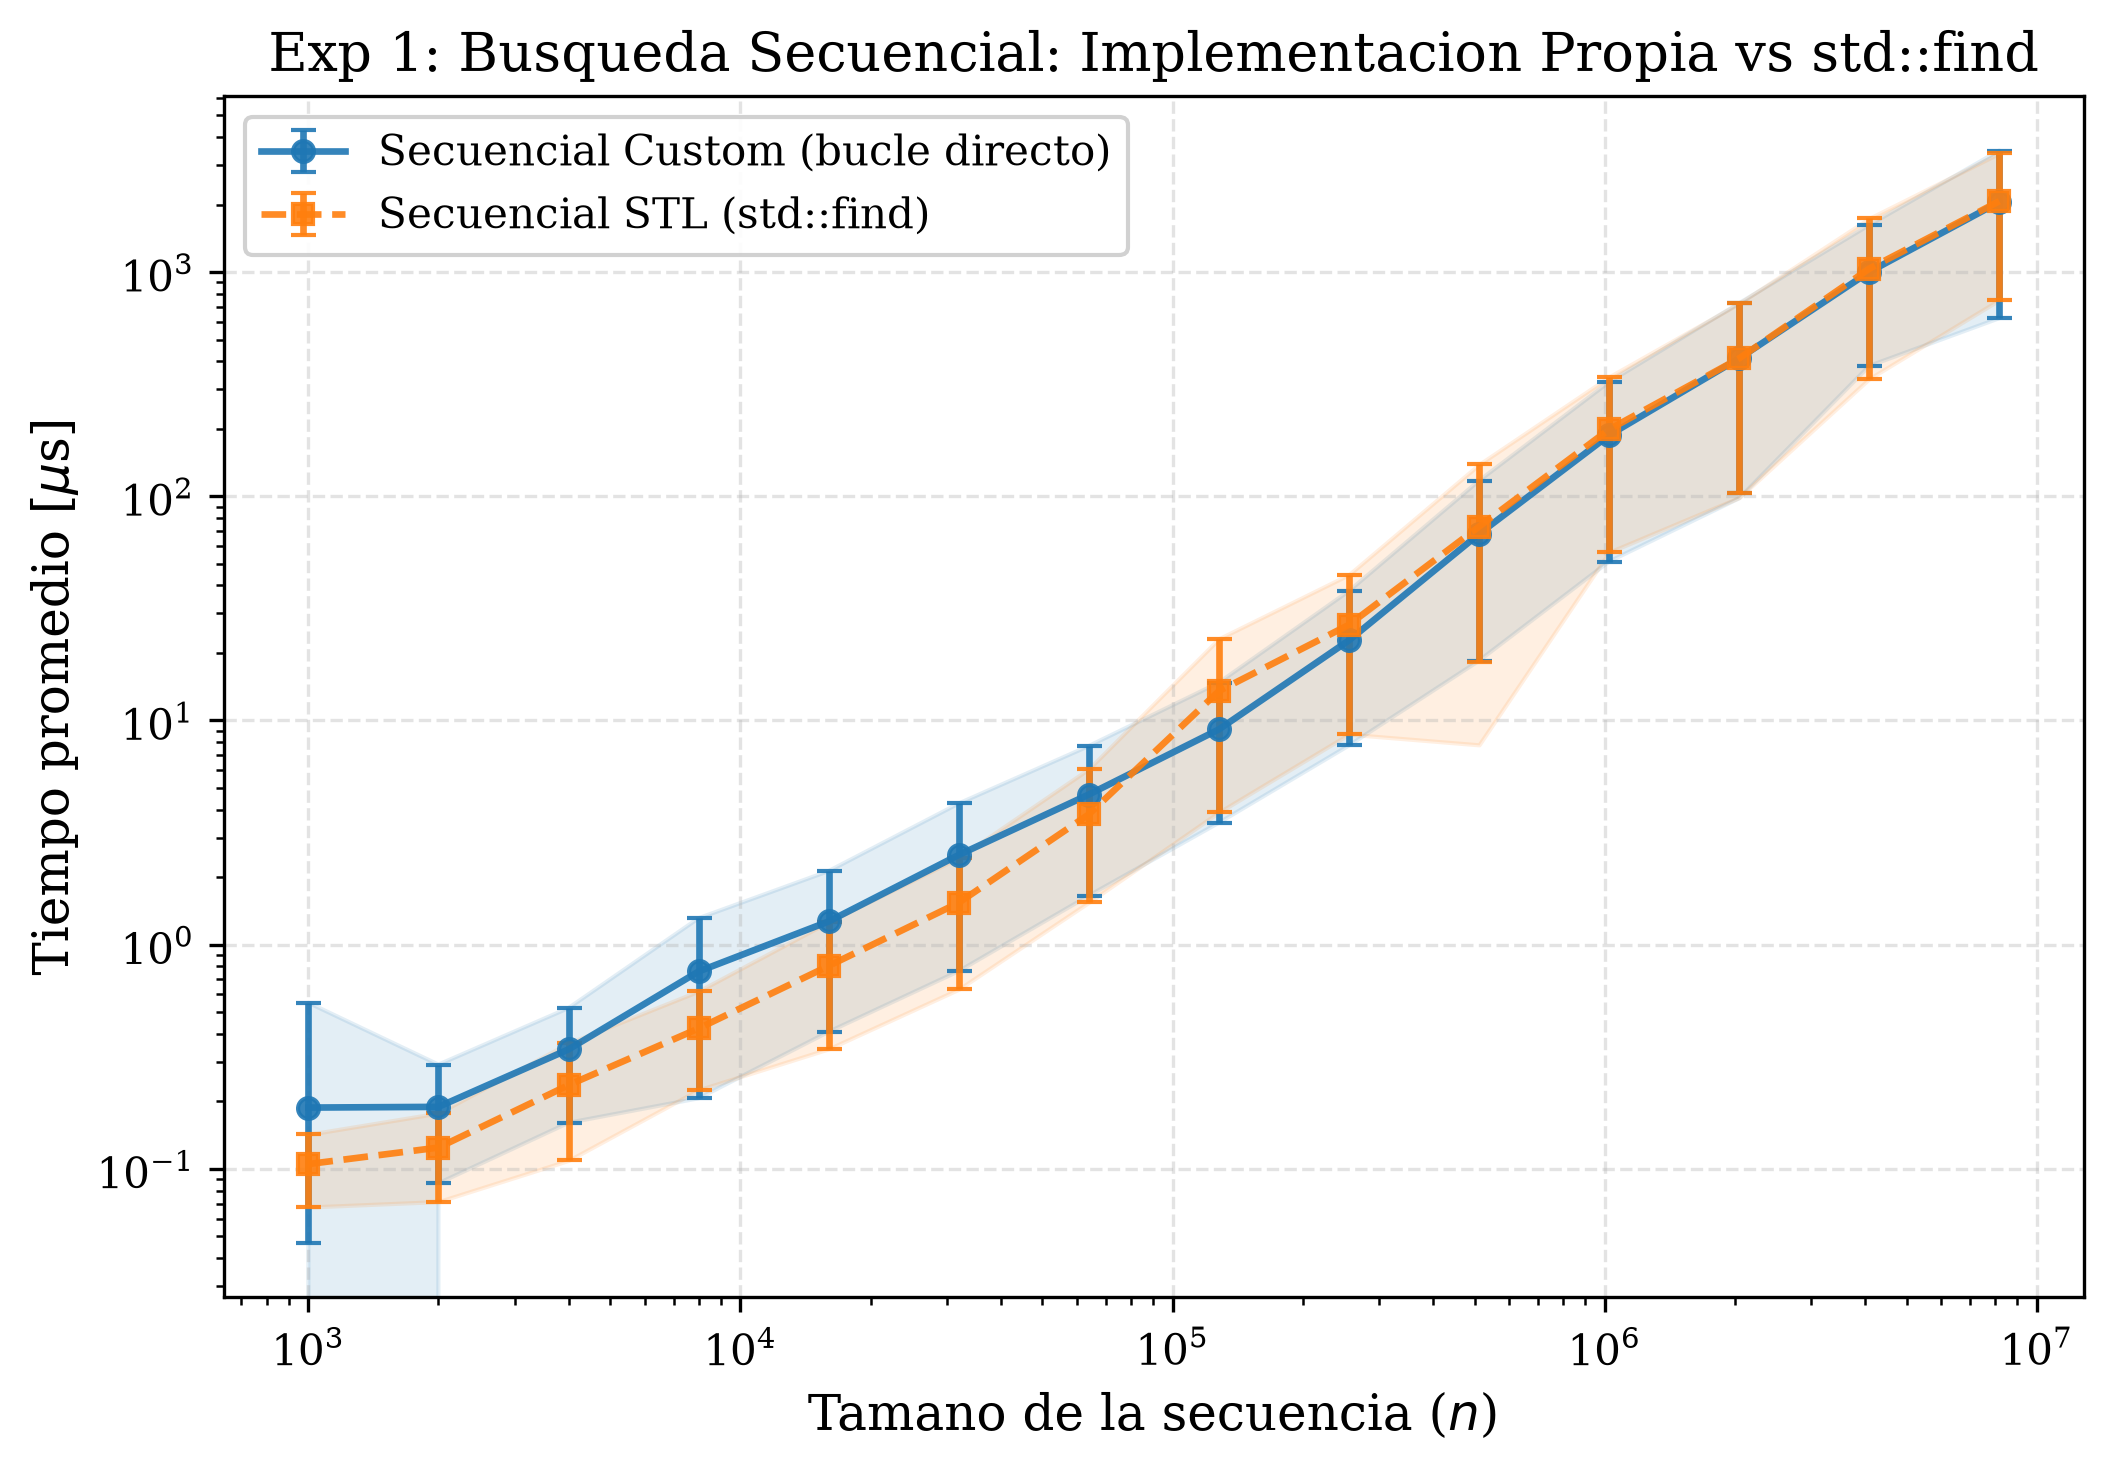
\includegraphics[width=\textwidth]{../plots/Experimento_1_Size/fig_size_seq_vs_stl.png}
        \caption{Secuencial Custom vs \texttt{std::find}.}
        \label{fig:size_seq}
    \end{subfigure}
    \hfill
    \begin{subfigure}[b]{0.48\textwidth}
        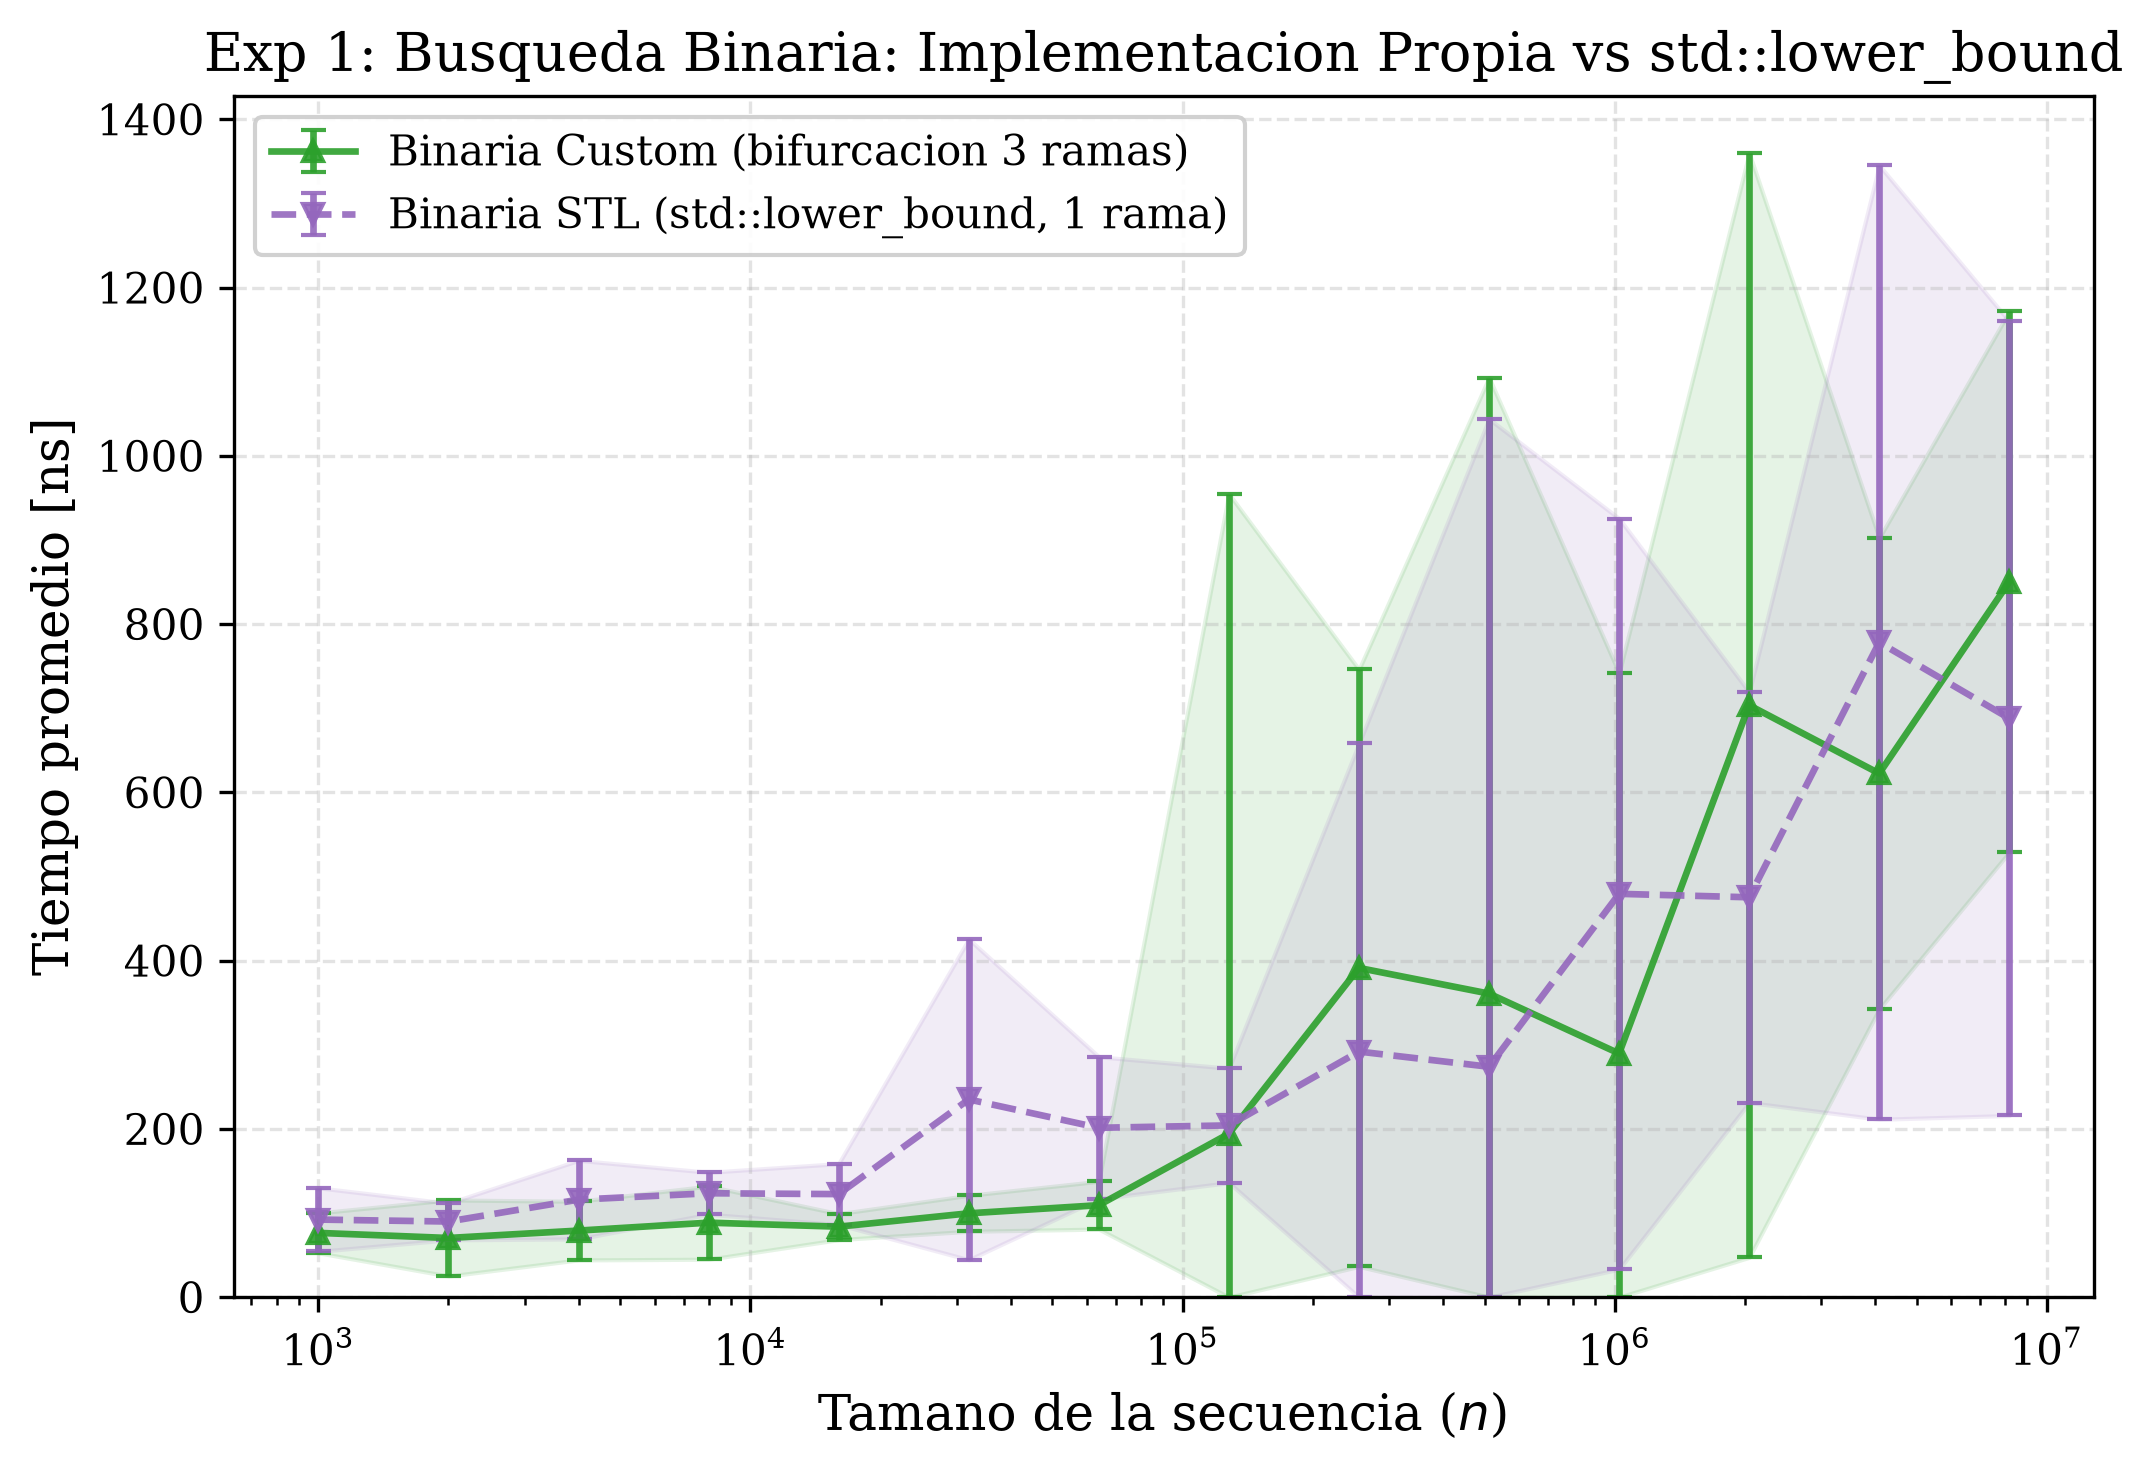
\includegraphics[width=\textwidth]{../plots/Experimento_1_Size/fig_size_bin_vs_stl.png}
        \caption{Binaria Custom vs \texttt{std::lower\_bound}.}
        \label{fig:size_bin}
    \end{subfigure}
    \vskip\baselineskip
    \begin{subfigure}[b]{0.48\textwidth}
        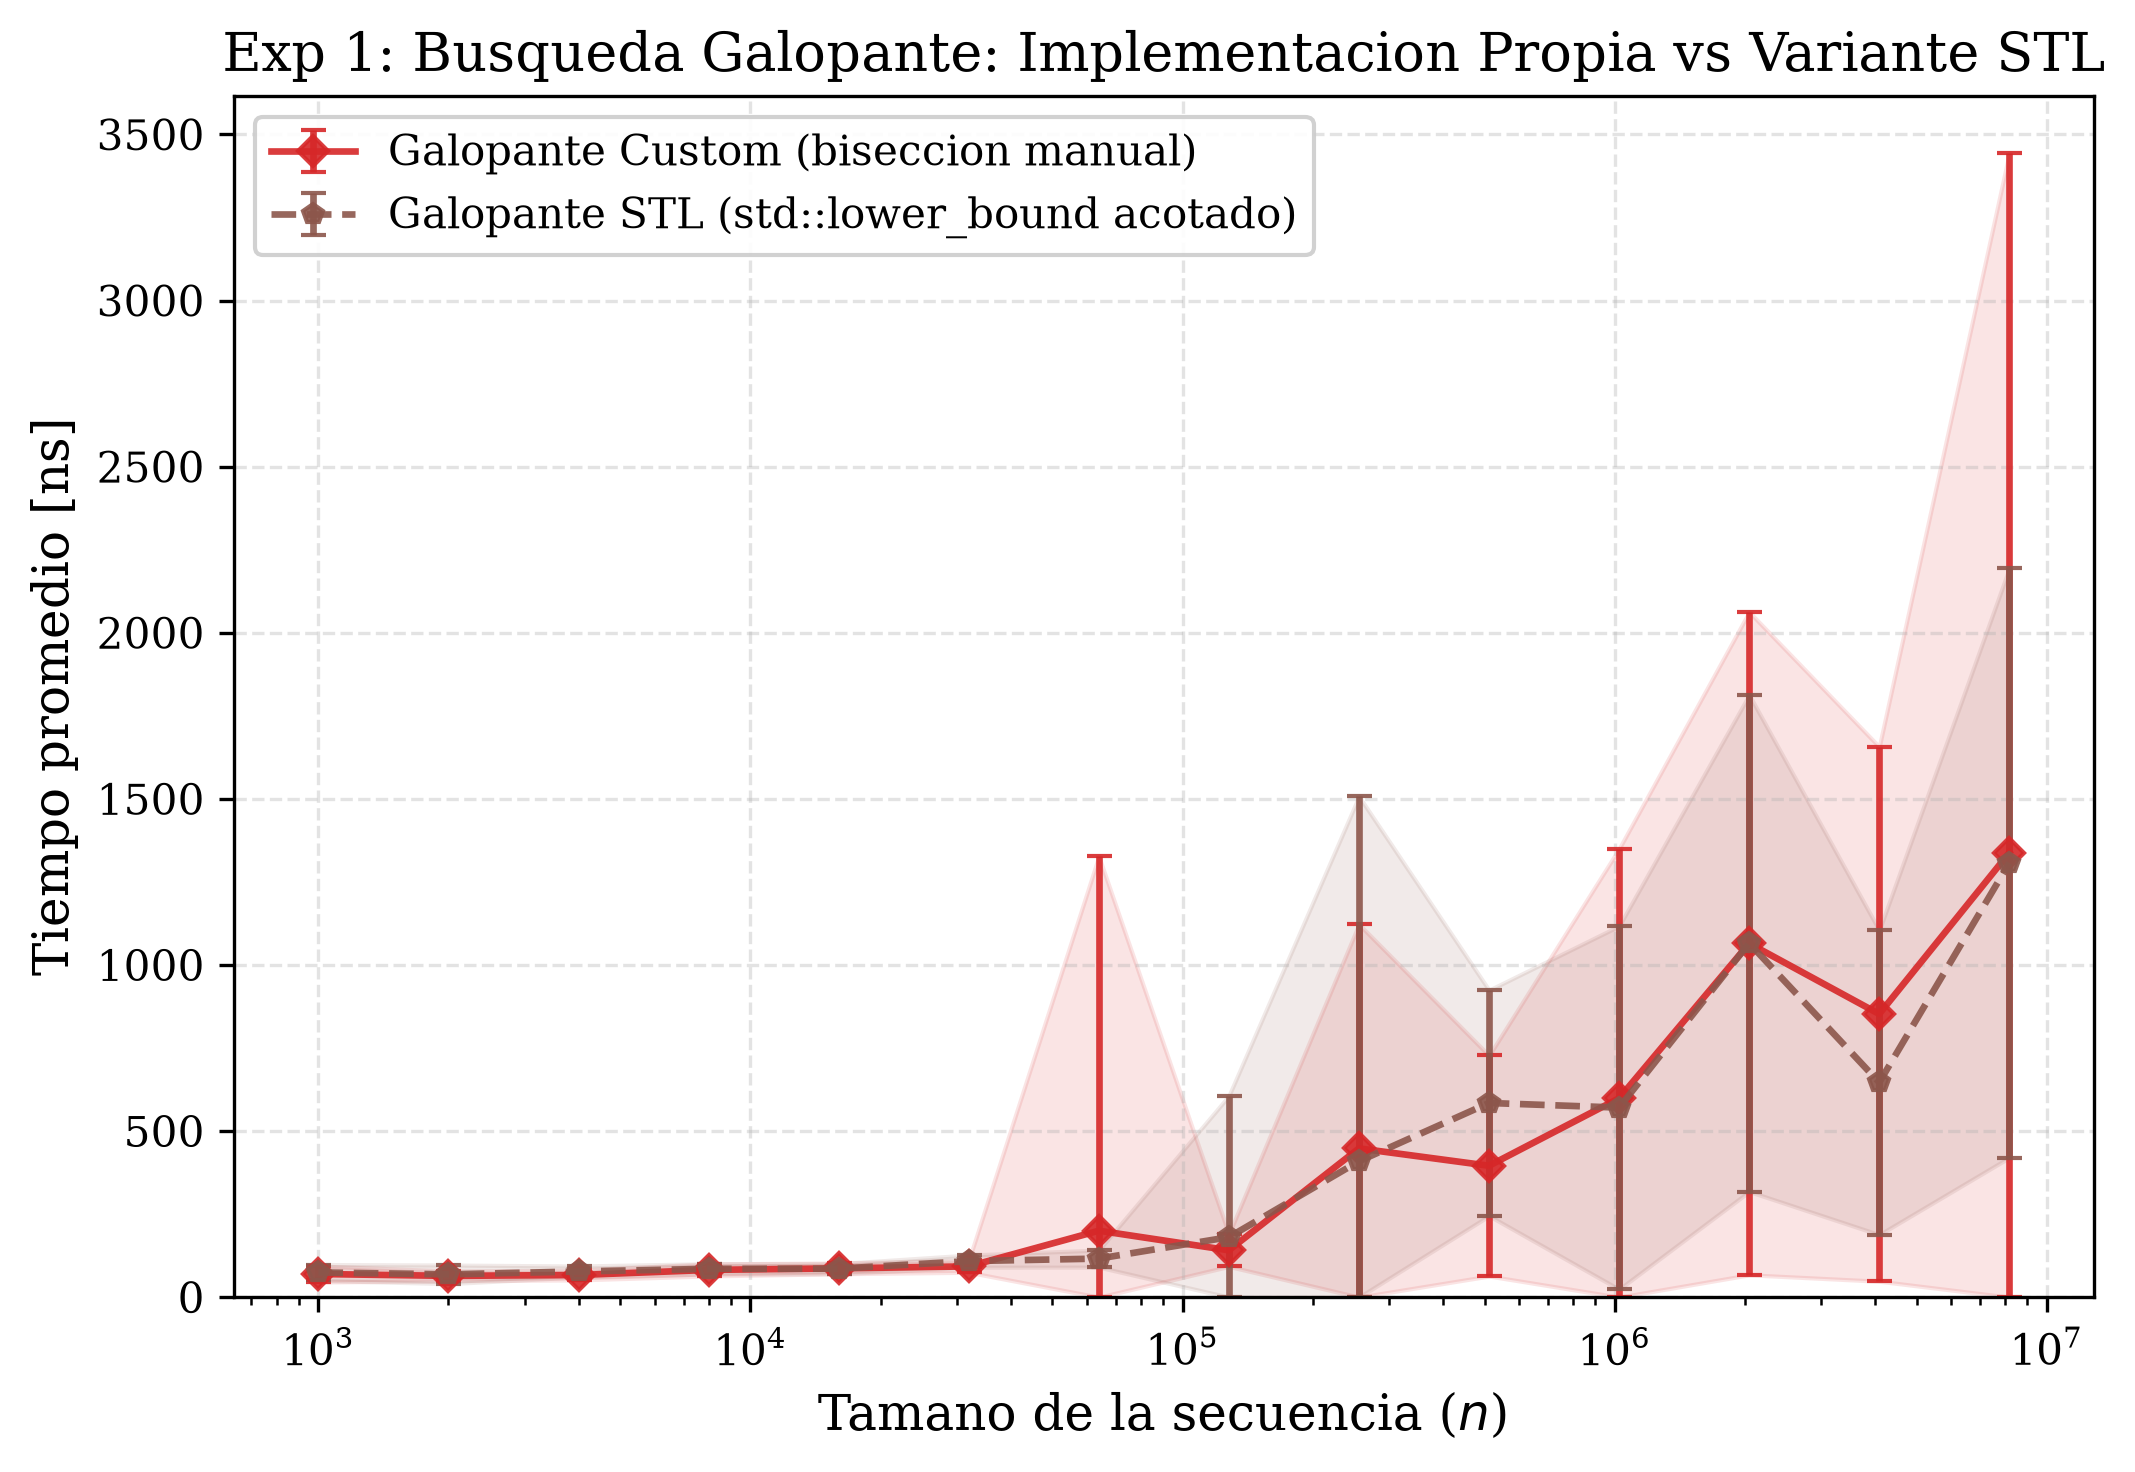
\includegraphics[width=\textwidth]{../plots/Experimento_1_Size/fig_size_gal_vs_stl.png}
        \caption{Galopante Custom vs Variante STL.}
        \label{fig:size_gal}
    \end{subfigure}
    \hfill
    \begin{subfigure}[b]{0.48\textwidth}
        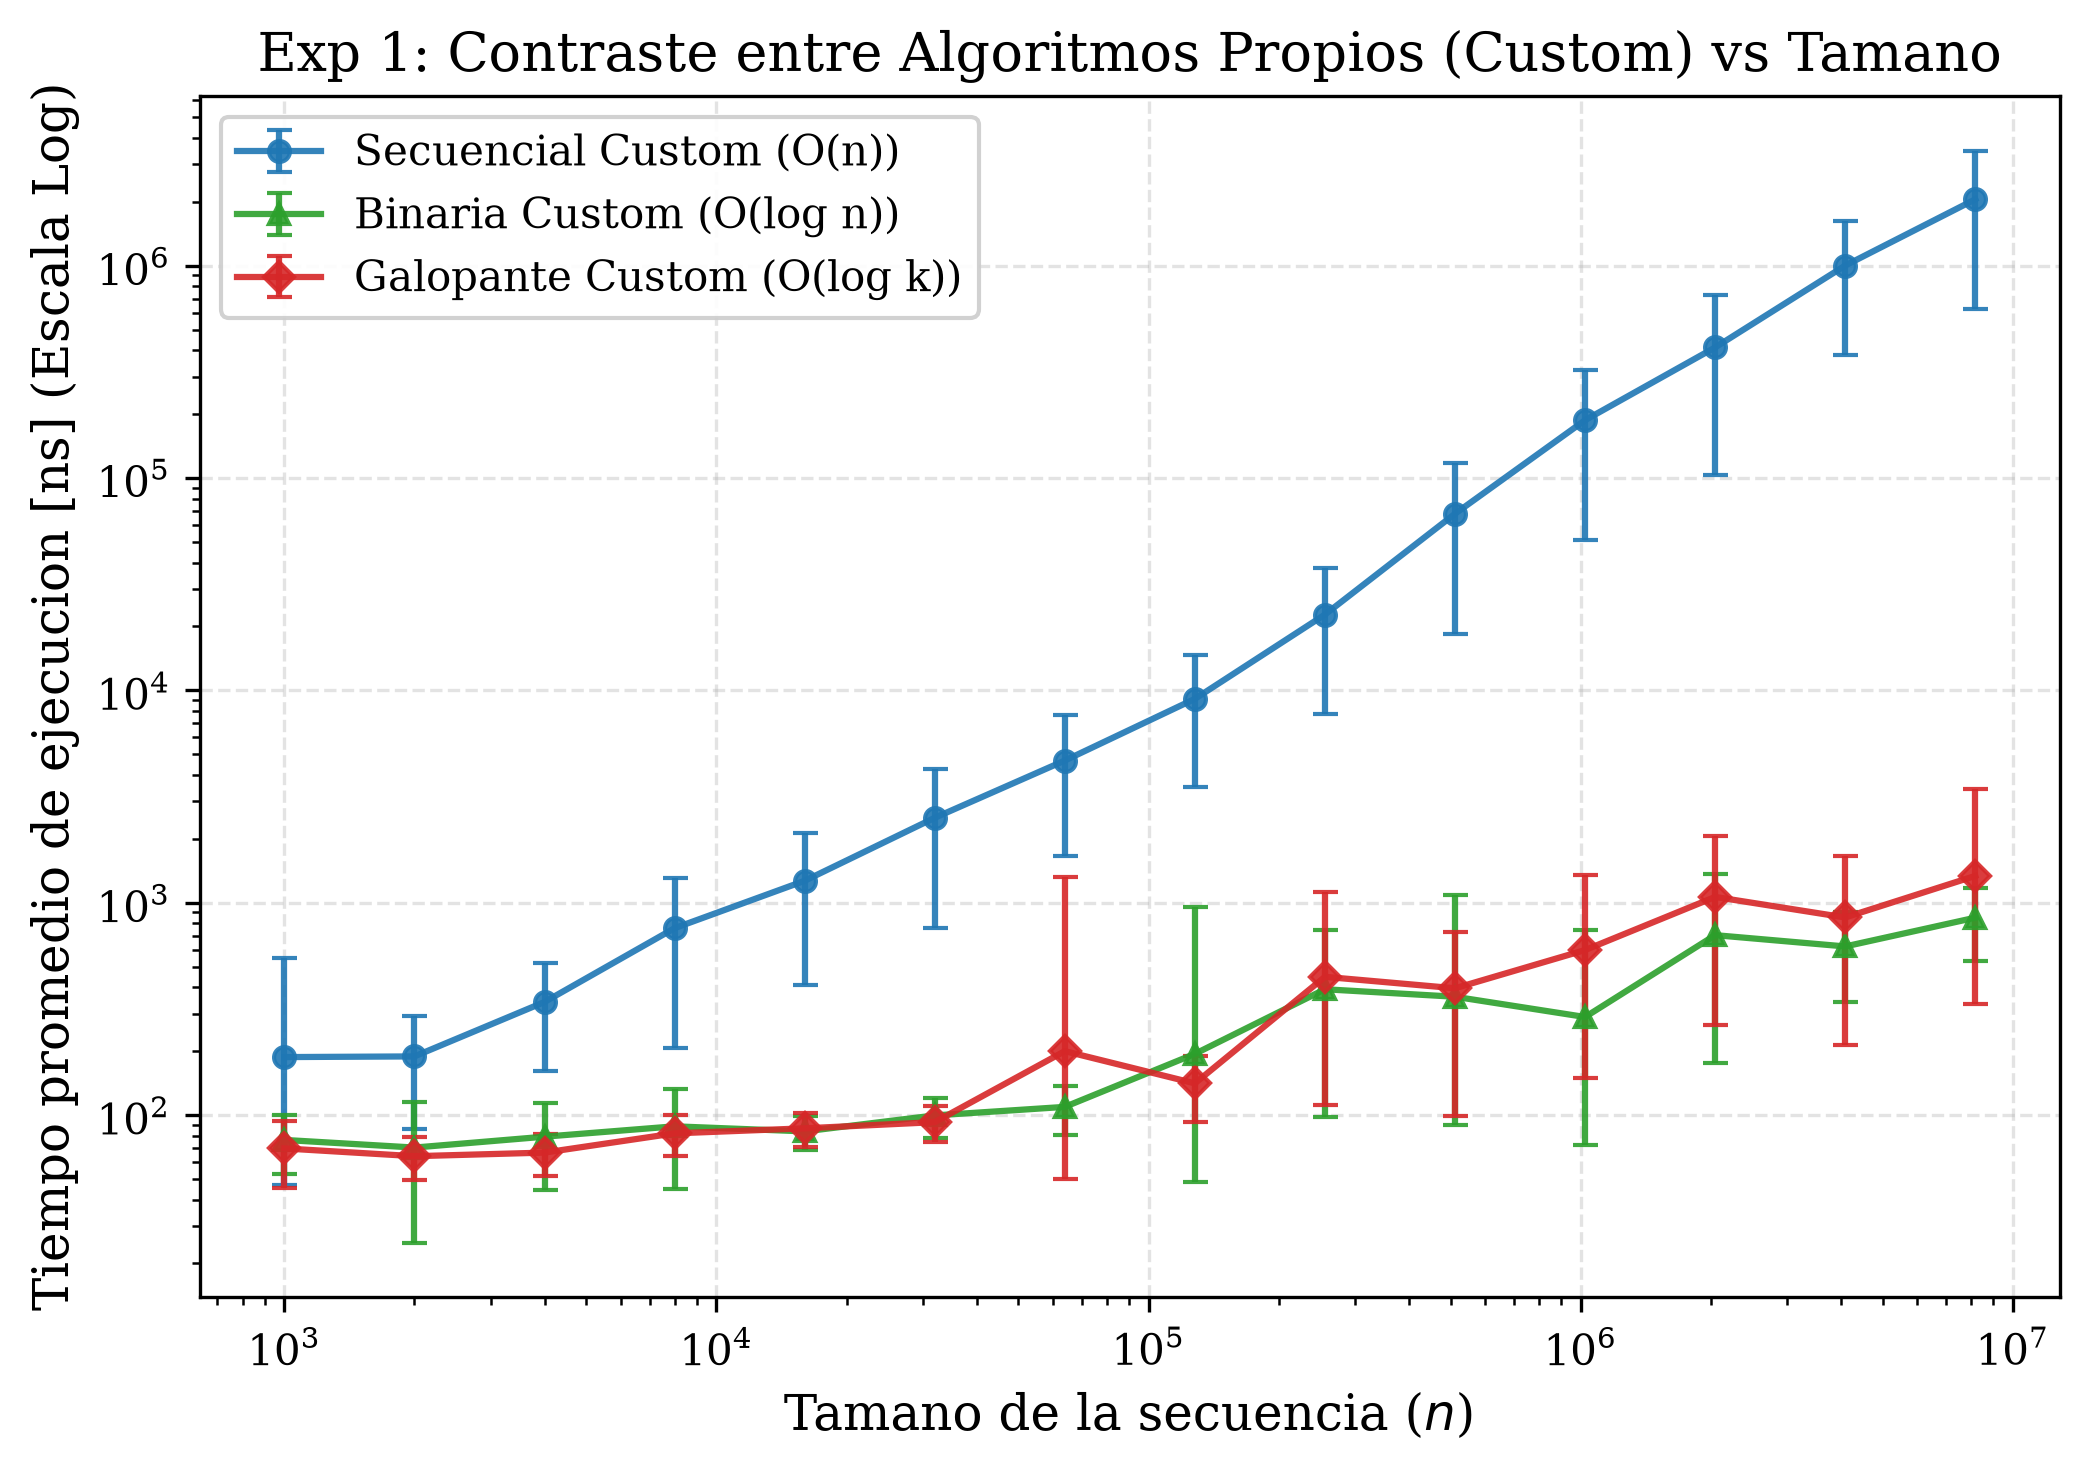
\includegraphics[width=\textwidth]{../plots/Experimento_1_Size/fig_size_custom_all.png}
        \caption{Contraste Global entre Algoritmos Propios.}
        \label{fig:size_all}
    \end{subfigure}
    \caption{Experimento 1: Tiempos promedio en función del tamaño de la secuencia ($n$).}
    \label{fig:exp1_size}
\end{figure}

\paragraph{Observaciones.}
\begin{itemize}
    \item \textbf{Secuencial vs.\ STL (Fig.~\ref{fig:size_seq}):} Ambas curvas crecen linealmente con $n$. En tamaños pequeños ($n \le 64\,000$), la STL registra menores tiempos ($422\text{ ns}$ vs $758\text{ ns}$ en $n = 8\,000$). Hacia $n = 8\,192\,000$ ambas convergen ($2.053\text{ ms}$ vs $2.070\text{ ms}$, diferencia $< 1\%$).
    \item \textbf{Binaria vs.\ STL (Fig.~\ref{fig:size_bin}):} La versión propia exhibe tiempos inferiores para $n \le 64\,000$ ($\approx 76\text{ ns}$ vs $\approx 92\text{ ns}$). A partir de $n \ge 128\,000$, ambas variantes presentan dispersión creciente y tiempos similares ($\approx 200\text{--}850\text{ ns}$).
    \item \textbf{Galopante vs.\ STL (Fig.~\ref{fig:size_gal}):} Ambas curvas coinciden a lo largo del dominio completo ($\approx 70\text{ ns}$ en $n=1\,000$ hasta $\approx 1\,337\text{ ns}$ en $n=8\,192\,000$).
    \item \textbf{Contraste Custom (Fig.~\ref{fig:size_all}):} La secuencial se separa en varios órdenes de magnitud ($2.05\text{ ms}$ en $n = 8\,192\,000$) respecto a binaria ($850\text{ ns}$) y galopante ($1\,337\text{ ns}$). La búsqueda binaria se mantiene por debajo de la galopante para todos los tamaños.
\end{itemize}


\subsubsection{Experimento 2: Variación por Posición del Objetivo ($k$)}

Se fijó una secuencia ordenada de tamaño masivo $N = 10\,000\,001$ elementos ($\approx 80\text{ MB}$, superando holgadamente la memoria caché L3) y se evaluó el tiempo de búsqueda variando la posición relativa $k$ entre $0$ y $10\,000\,000$. 

\paragraph{Justificación del muestreo de $k$:}
En lugar de un barrido unitario ($k = 0, 1, 2, \dots, 10^7$) ---el cual resultaría computacionalmente intratable, requiriendo más de 38 días continuos de cómputo solo para la búsqueda secuencial ($1.28 \times 10^9$ ejecuciones acumuladas) y siendo estadísticamente redundante debido a la suavidad y monotonía de las curvas subyacentes---, se diseñó un muestreo sistemático de 21 puntos equiespaciados con un paso aditivo de $\Delta k = 500\,000$ (incrementos exactos del $5\%$ del arreglo). Con $M = 128$ repeticiones por cada punto de muestreo, el Teorema del Límite Central garantiza una caracterización empírica de alta fidelidad con un costo de cómputo razonable.

% --- HIPÓTESIS EXPERIMENTO 2 ---
\paragraph{Hipótesis.}
Se espera que la búsqueda secuencial presente una relación estrictamente proporcional a $k$, creciendo linealmente con la posición del objetivo. La búsqueda binaria debería mostrarse invariante respecto a la posición, ya que siempre parte desde el punto medio. La búsqueda galopante debería exhibir tiempos mínimos en posiciones cercanas al inicio ($k \ll N$), superando incluso a la binaria, dado que su complejidad $\mathcal{O}(\log k)$ se traduce en pocos saltos exponenciales cuando $k$ es pequeño.

\begin{figure}[H]
    \centering
    \begin{subfigure}[b]{0.48\textwidth}
        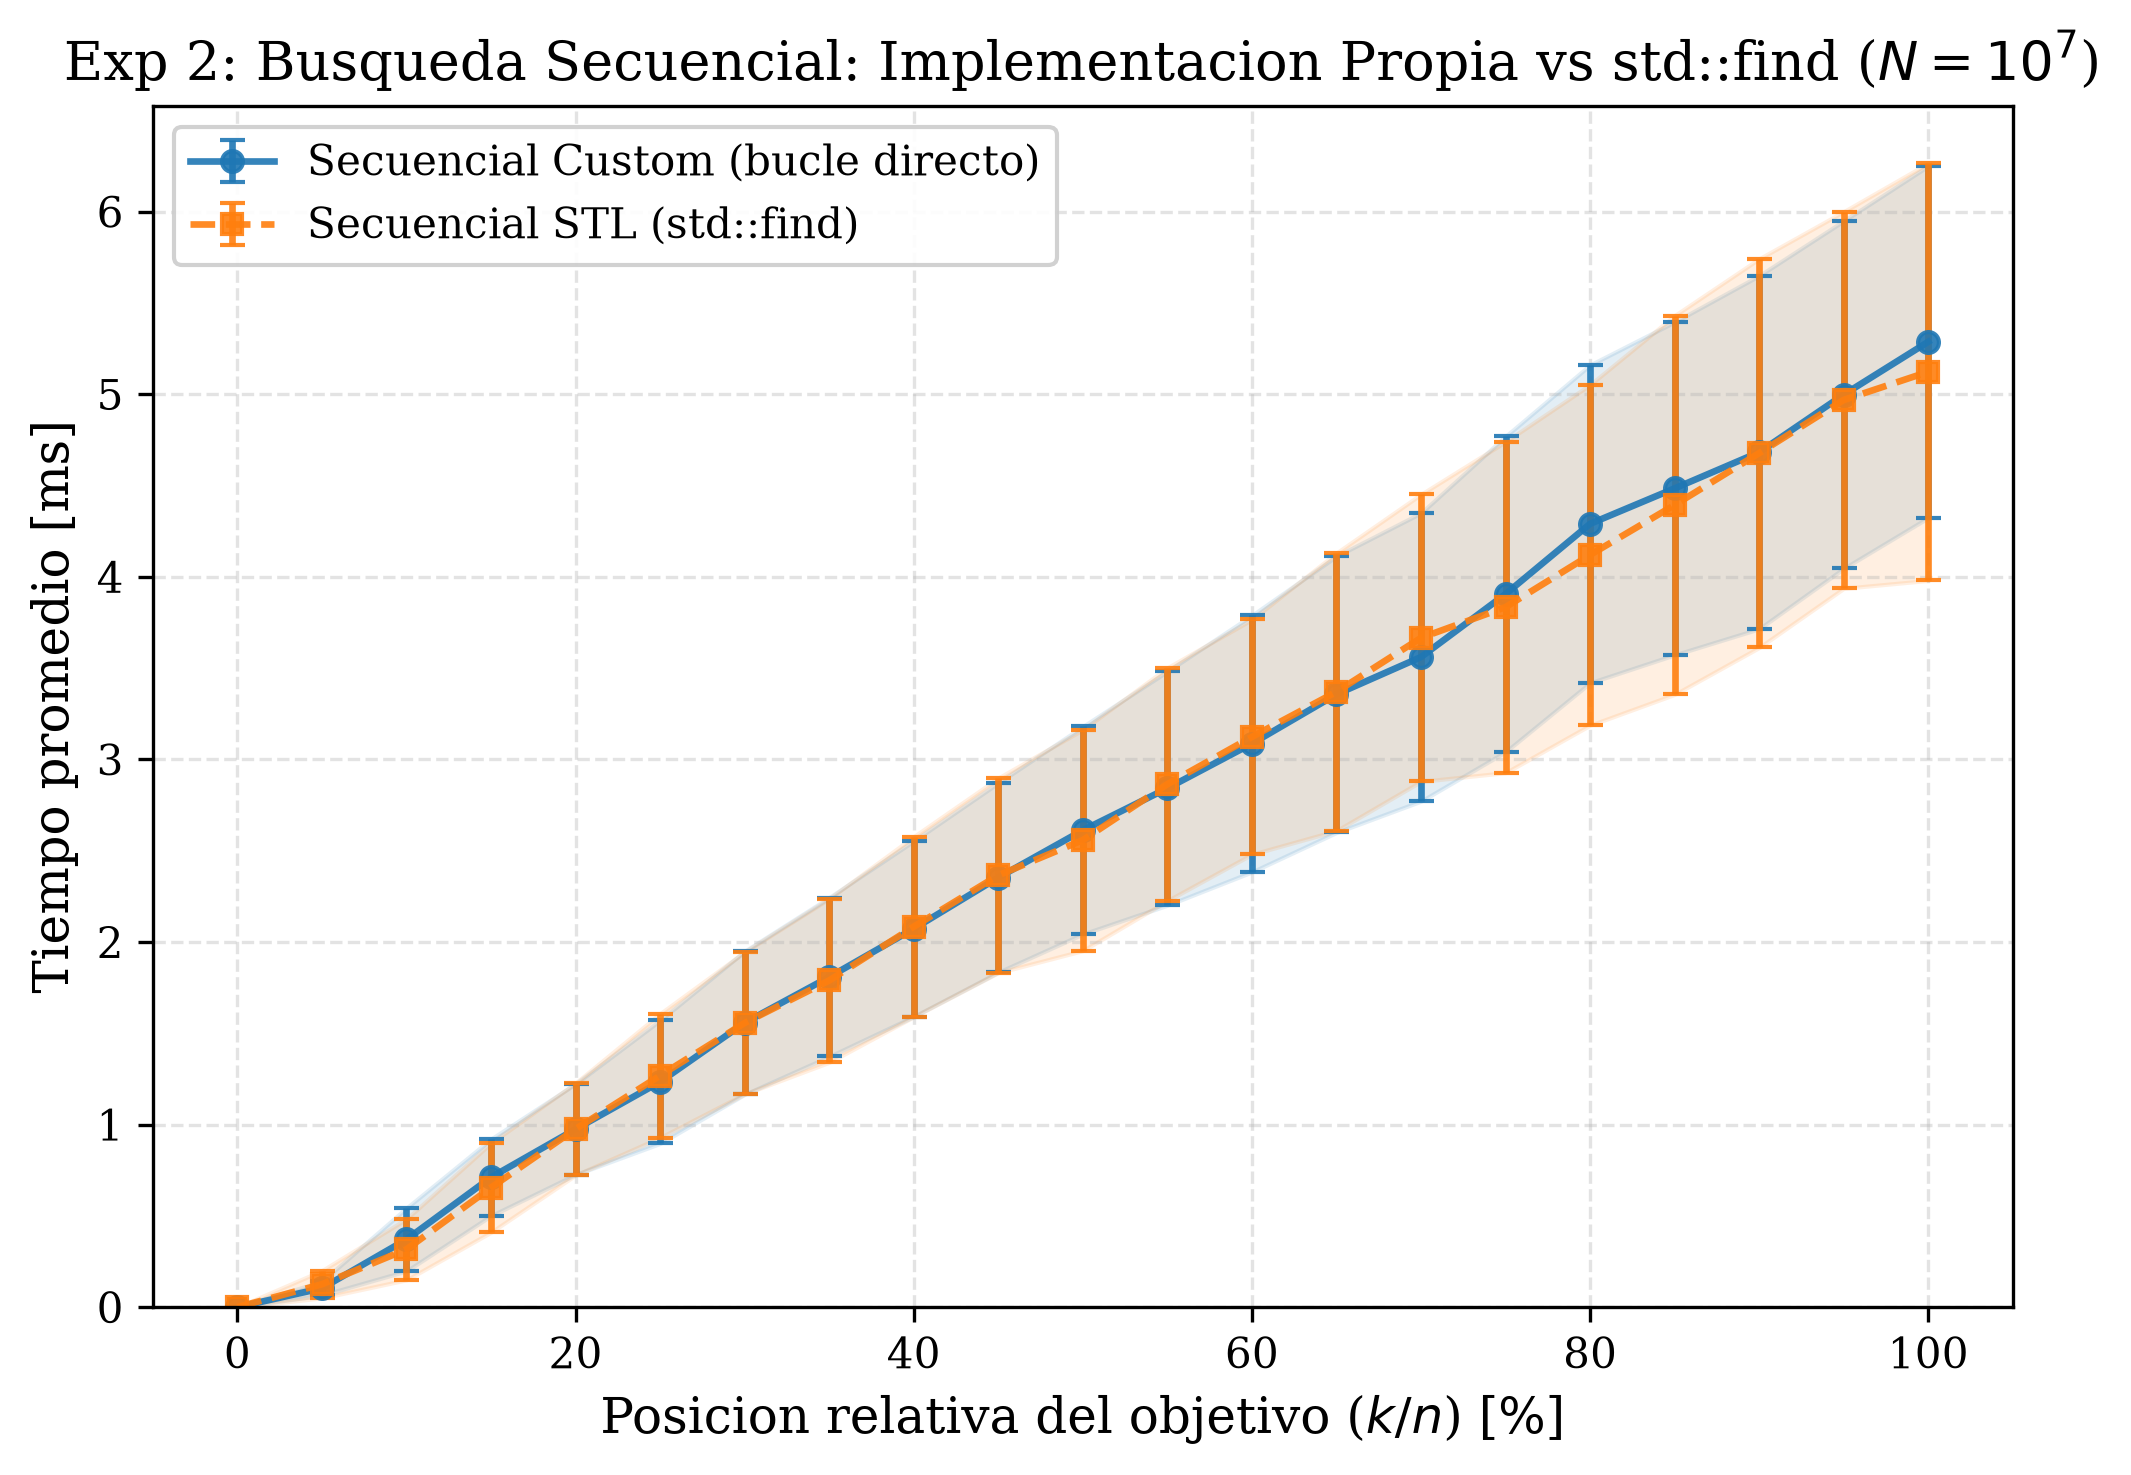
\includegraphics[width=\textwidth]{../plots/Experimento_2_Posicion/fig_pos_seq_vs_stl.png}
        \caption{Secuencial Custom vs STL.}
        \label{fig:pos_seq}
    \end{subfigure}
    \hfill
    \begin{subfigure}[b]{0.48\textwidth}
        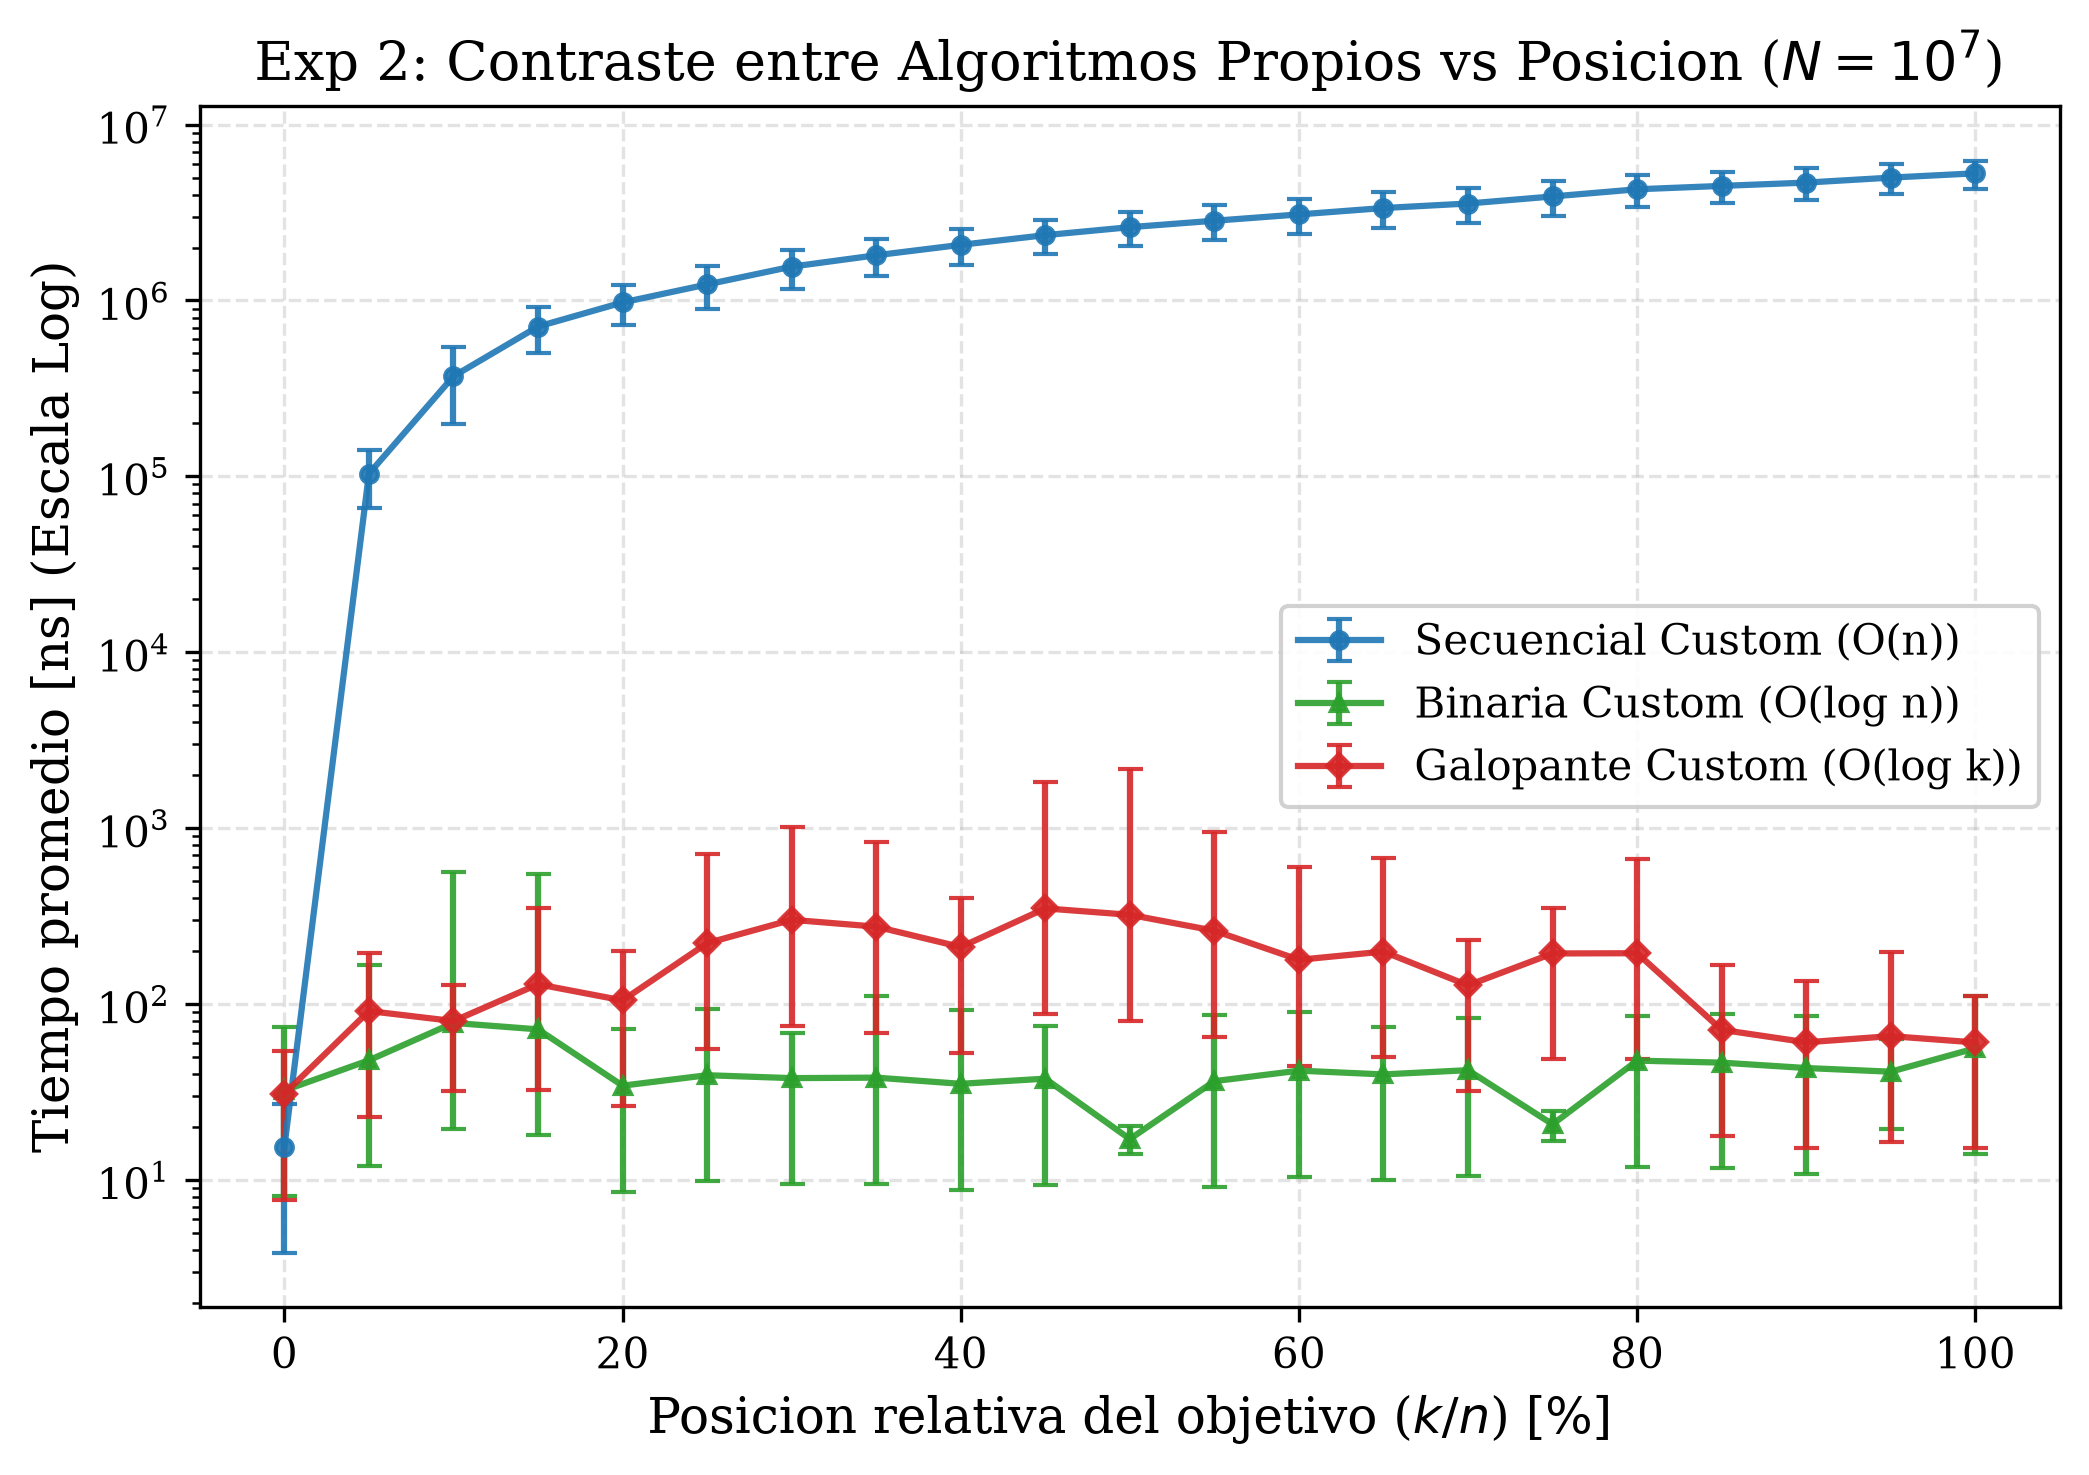
\includegraphics[width=\textwidth]{../plots/Experimento_2_Posicion/fig_pos_custom_all.png}
        \caption{Contraste Global Algoritmos Propios.}
        \label{fig:pos_all}
    \end{subfigure}
    \vskip\baselineskip
    \begin{subfigure}[b]{0.48\textwidth}
        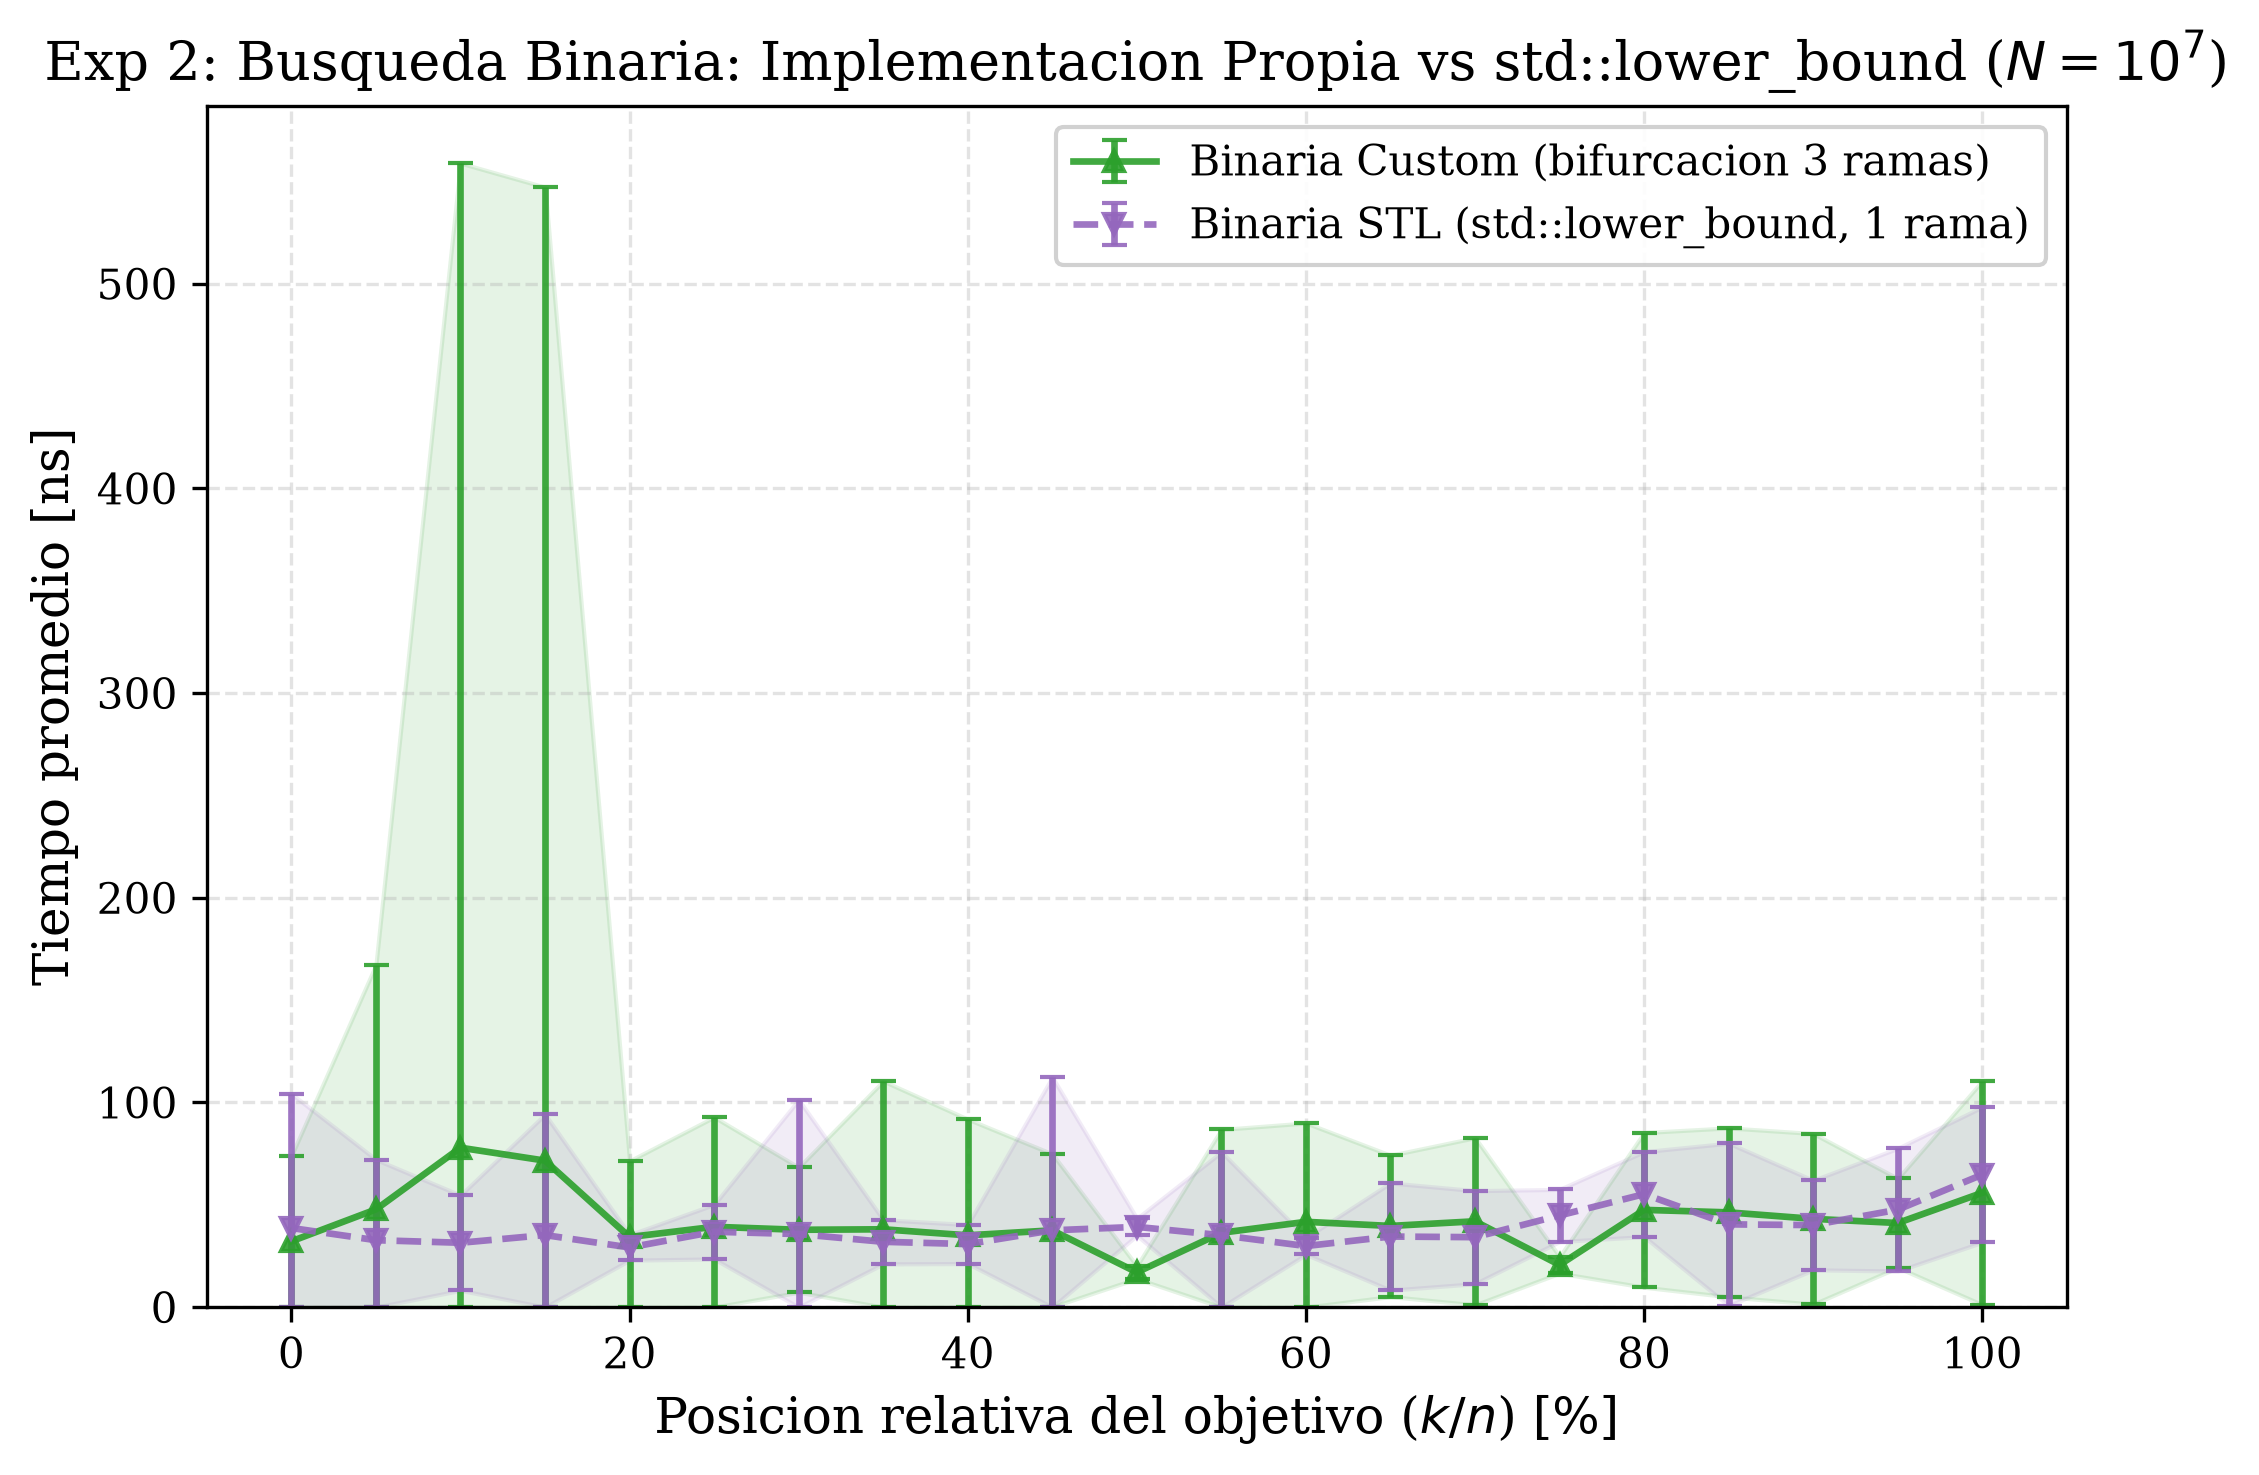
\includegraphics[width=\textwidth]{../plots/Experimento_2_Posicion/fig_pos_bin_vs_stl.png}
        \caption{Binaria Custom vs \texttt{std::lower\_bound}.}
        \label{fig:pos_bin}
    \end{subfigure}
    \hfill
    \begin{subfigure}[b]{0.48\textwidth}
        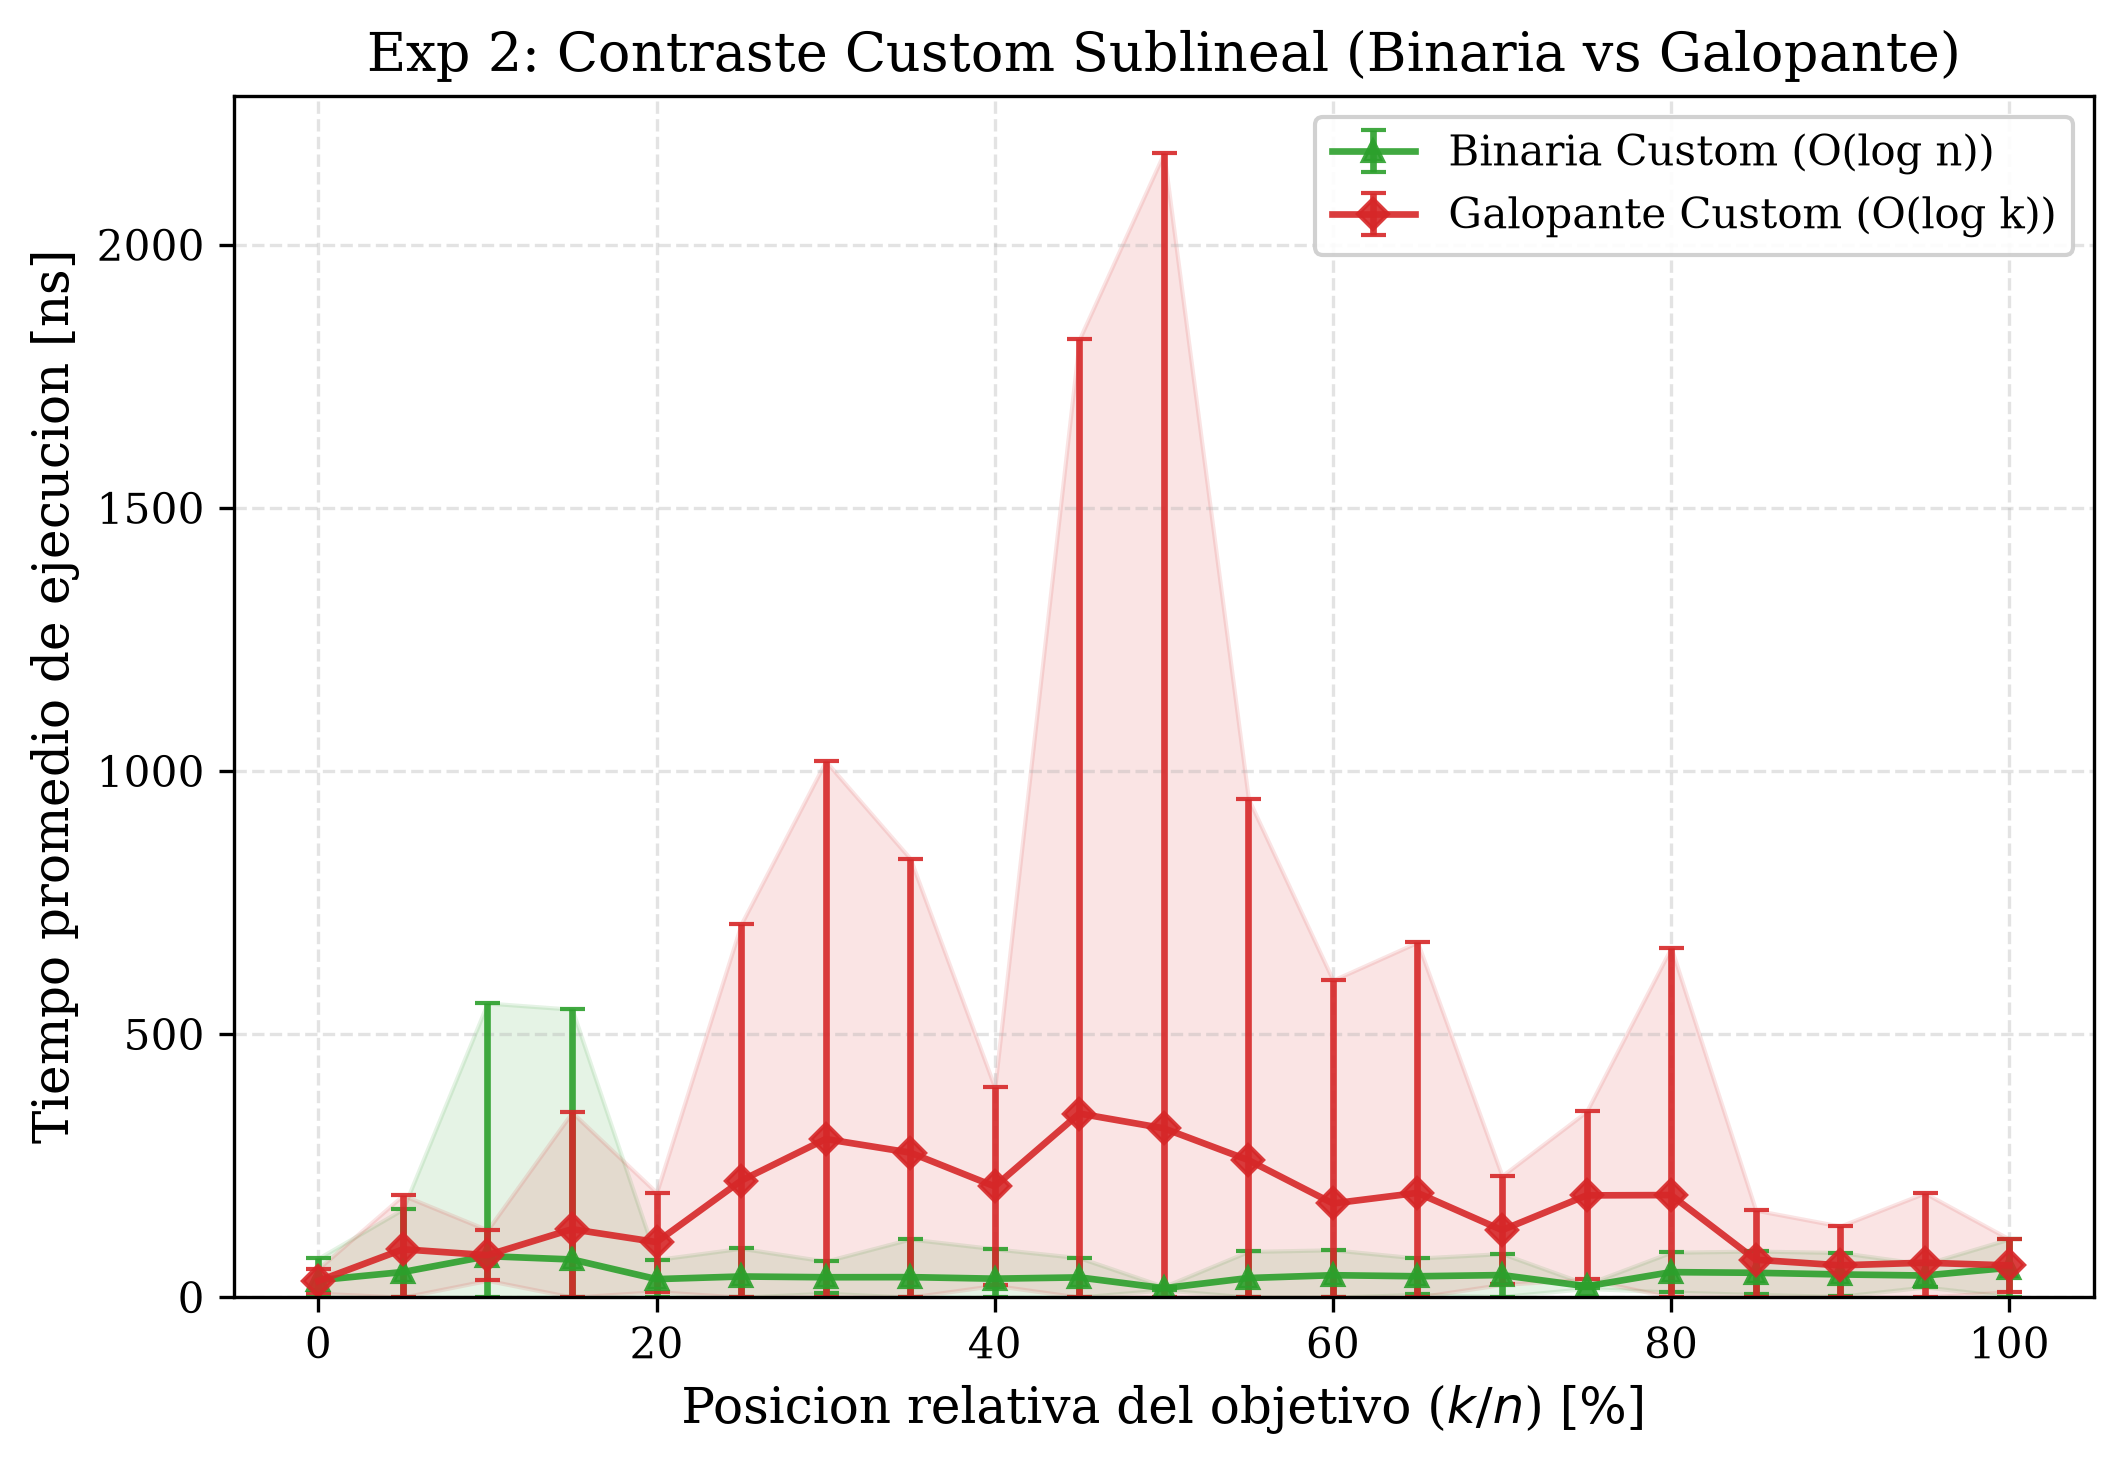
\includegraphics[width=\textwidth]{../plots/Experimento_2_Posicion/fig_pos_custom_bin_vs_gal.png}
        \caption{Binaria vs Galopante (Zoom Sublineal).}
        \label{fig:pos_bin_gal}
    \end{subfigure}
    \caption{Experimento 2: Tiempos en función de la posición relativa del objetivo ($k/N$).}
    \label{fig:exp2_pos}
\end{figure}

\paragraph{Observaciones.}
\begin{itemize}
    \item \textbf{Secuencial (Fig.~\ref{fig:pos_seq}):} Relación lineal directa con $k$. Registra $\approx 0.01\text{ ms}$ cerca de $k = 0$ y escala hasta $\approx 2.6\text{ ms}$ en $k \to N$.
    \item \textbf{Binaria (Fig.~\ref{fig:pos_bin}):} Respuesta temporal constante e independiente de la posición, oscilando en la meseta de $\approx 17\text{--}56\text{ ns}$.
    \item \textbf{Galopante (Fig.~\ref{fig:pos_bin_gal}):} Registra tiempos mínimos en posiciones iniciales ($k/N \le 5\%$, $\approx 31\text{--}90\text{ ns}$). A partir de posiciones medias ($k/N \approx 25\%\text{--}60\%$), los tiempos aumentan y superan a la búsqueda binaria ($\approx 200\text{--}350\text{ ns}$ vs $\approx 35\text{--}48\text{ ns}$). En el extremo final ($k/N > 85\%$), la galopante vuelve a descender ($\approx 60\text{--}71\text{ ns}$), ya que el galope se detiene rápidamente al exceder el tamaño del arreglo.
\end{itemize}

\newpage

\subsubsection{Experimento 3: Colas de Prioridad (Heaps)}

Se contrastaron las cinco operaciones fundamentales entre Binary Heap y Binomial Heap, variando $n$ desde $1\,000$ hasta $512\,000$ elementos.

% --- HIPÓTESIS EXPERIMENTO 3 ---
\paragraph{Hipótesis.}
Se espera que el Binary Heap supere al Binomial Heap en las operaciones individuales (\texttt{top}, \texttt{insert}, \texttt{extract\_min} y \texttt{build}) debido a su representación contigua en memoria, la cual maximiza la localidad espacial y el aprovechamiento de la caché del procesador. La excepción debería ser la operación de fusión (\texttt{meld}), donde el Binomial Heap, al operar mediante manipulación de punteros en tiempo $\mathcal{O}(\log n)$, debería exhibir una clara superioridad frente a la reconstrucción lineal $\mathcal{O}(n)$ del Binary Heap.

\begin{figure}[H]
    \centering
    \begin{subfigure}[b]{0.48\textwidth}
        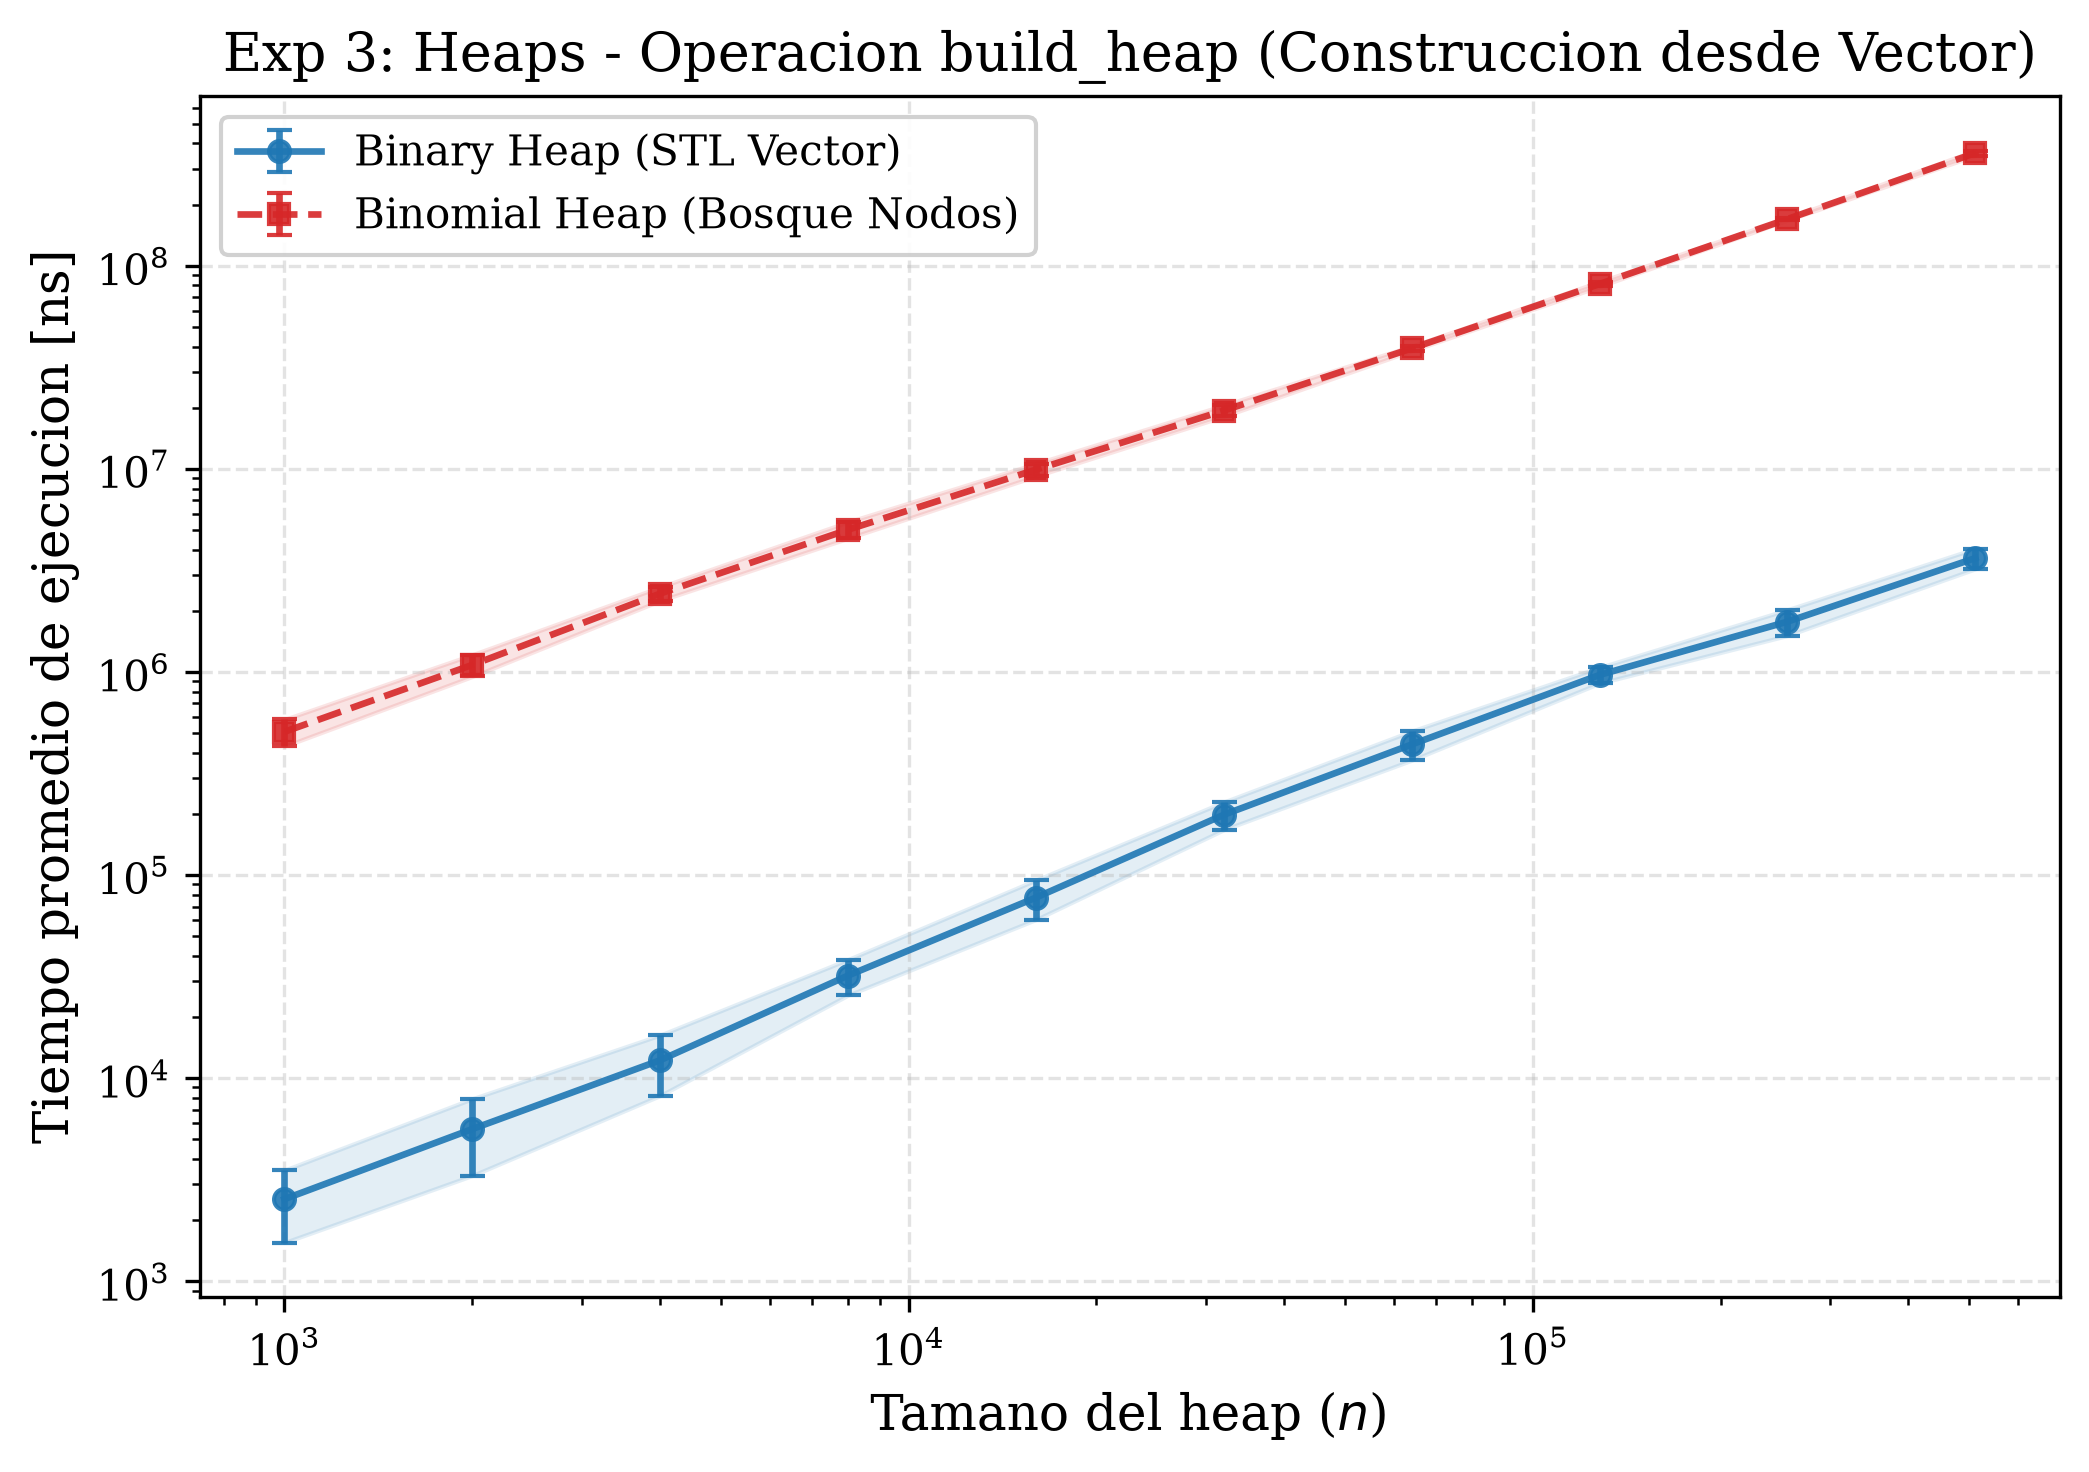
\includegraphics[width=\textwidth]{../plots/Experimento_3_Heaps/fig_heaps_build.png}
        \caption{\texttt{build\_heap}}
        \label{fig:heap_build}
    \end{subfigure}
    \hfill
    \begin{subfigure}[b]{0.48\textwidth}
        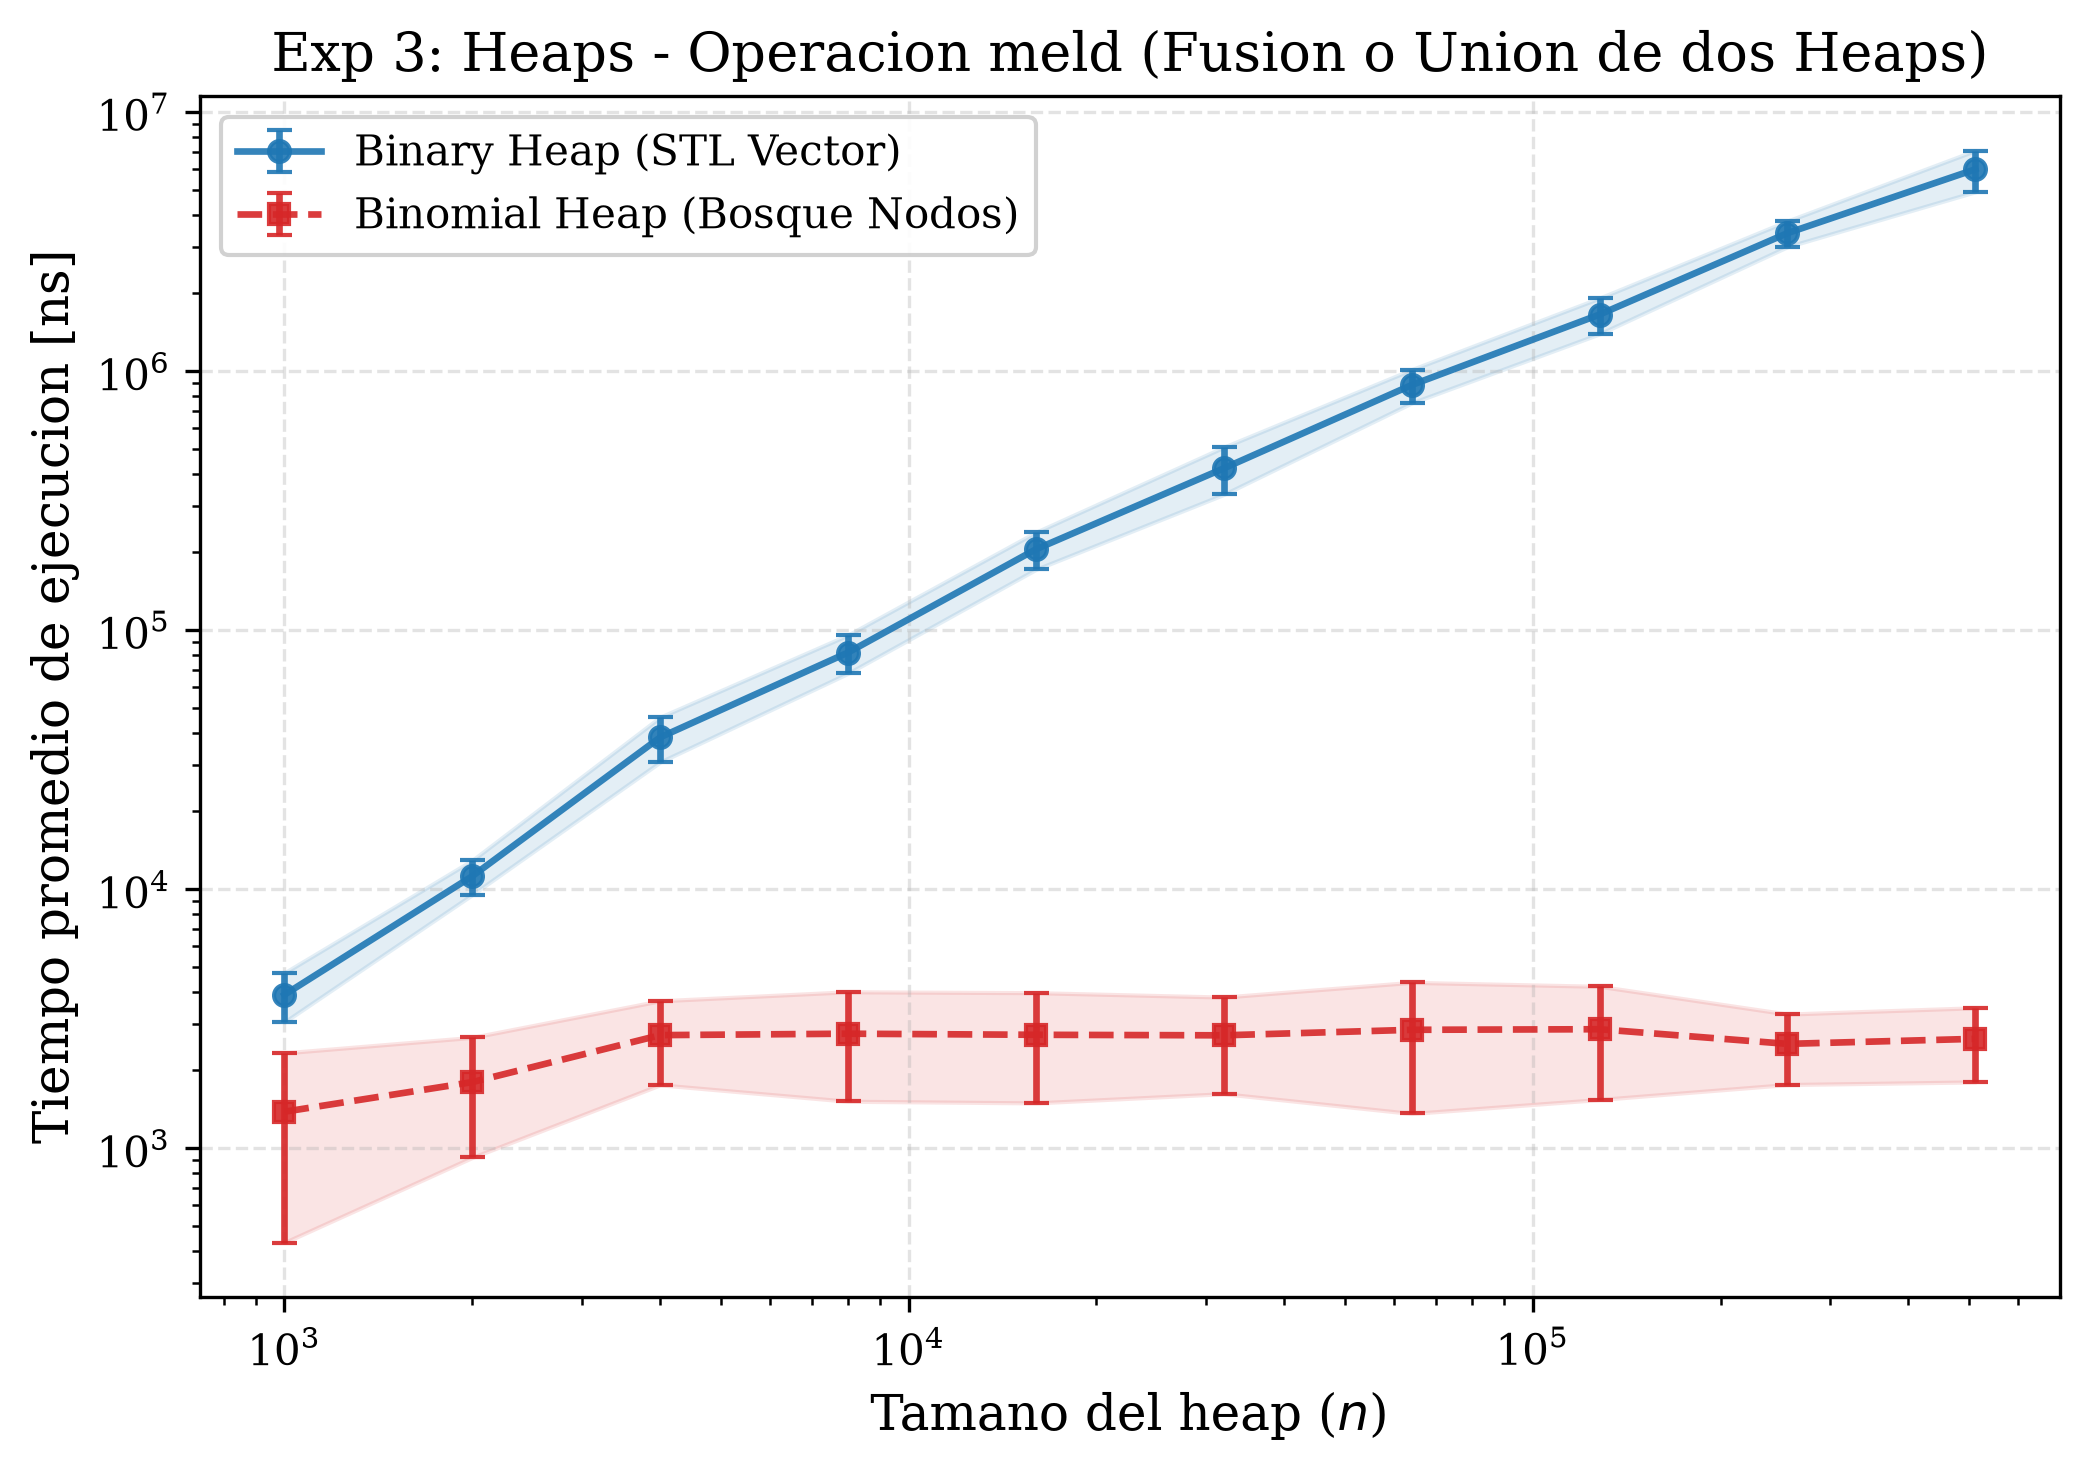
\includegraphics[width=\textwidth]{../plots/Experimento_3_Heaps/fig_heaps_meld.png}
        \caption{\texttt{meld} (Fusión)}
        \label{fig:heap_meld}
    \end{subfigure}
    \caption{Experimento 3: Operaciones de lote y reestructuración (\texttt{build\_heap} y \texttt{meld}).}
    \label{fig:exp3_heaps_batch}
\end{figure}

\begin{figure}[H]
    \centering
    \begin{subfigure}[b]{0.48\textwidth}
        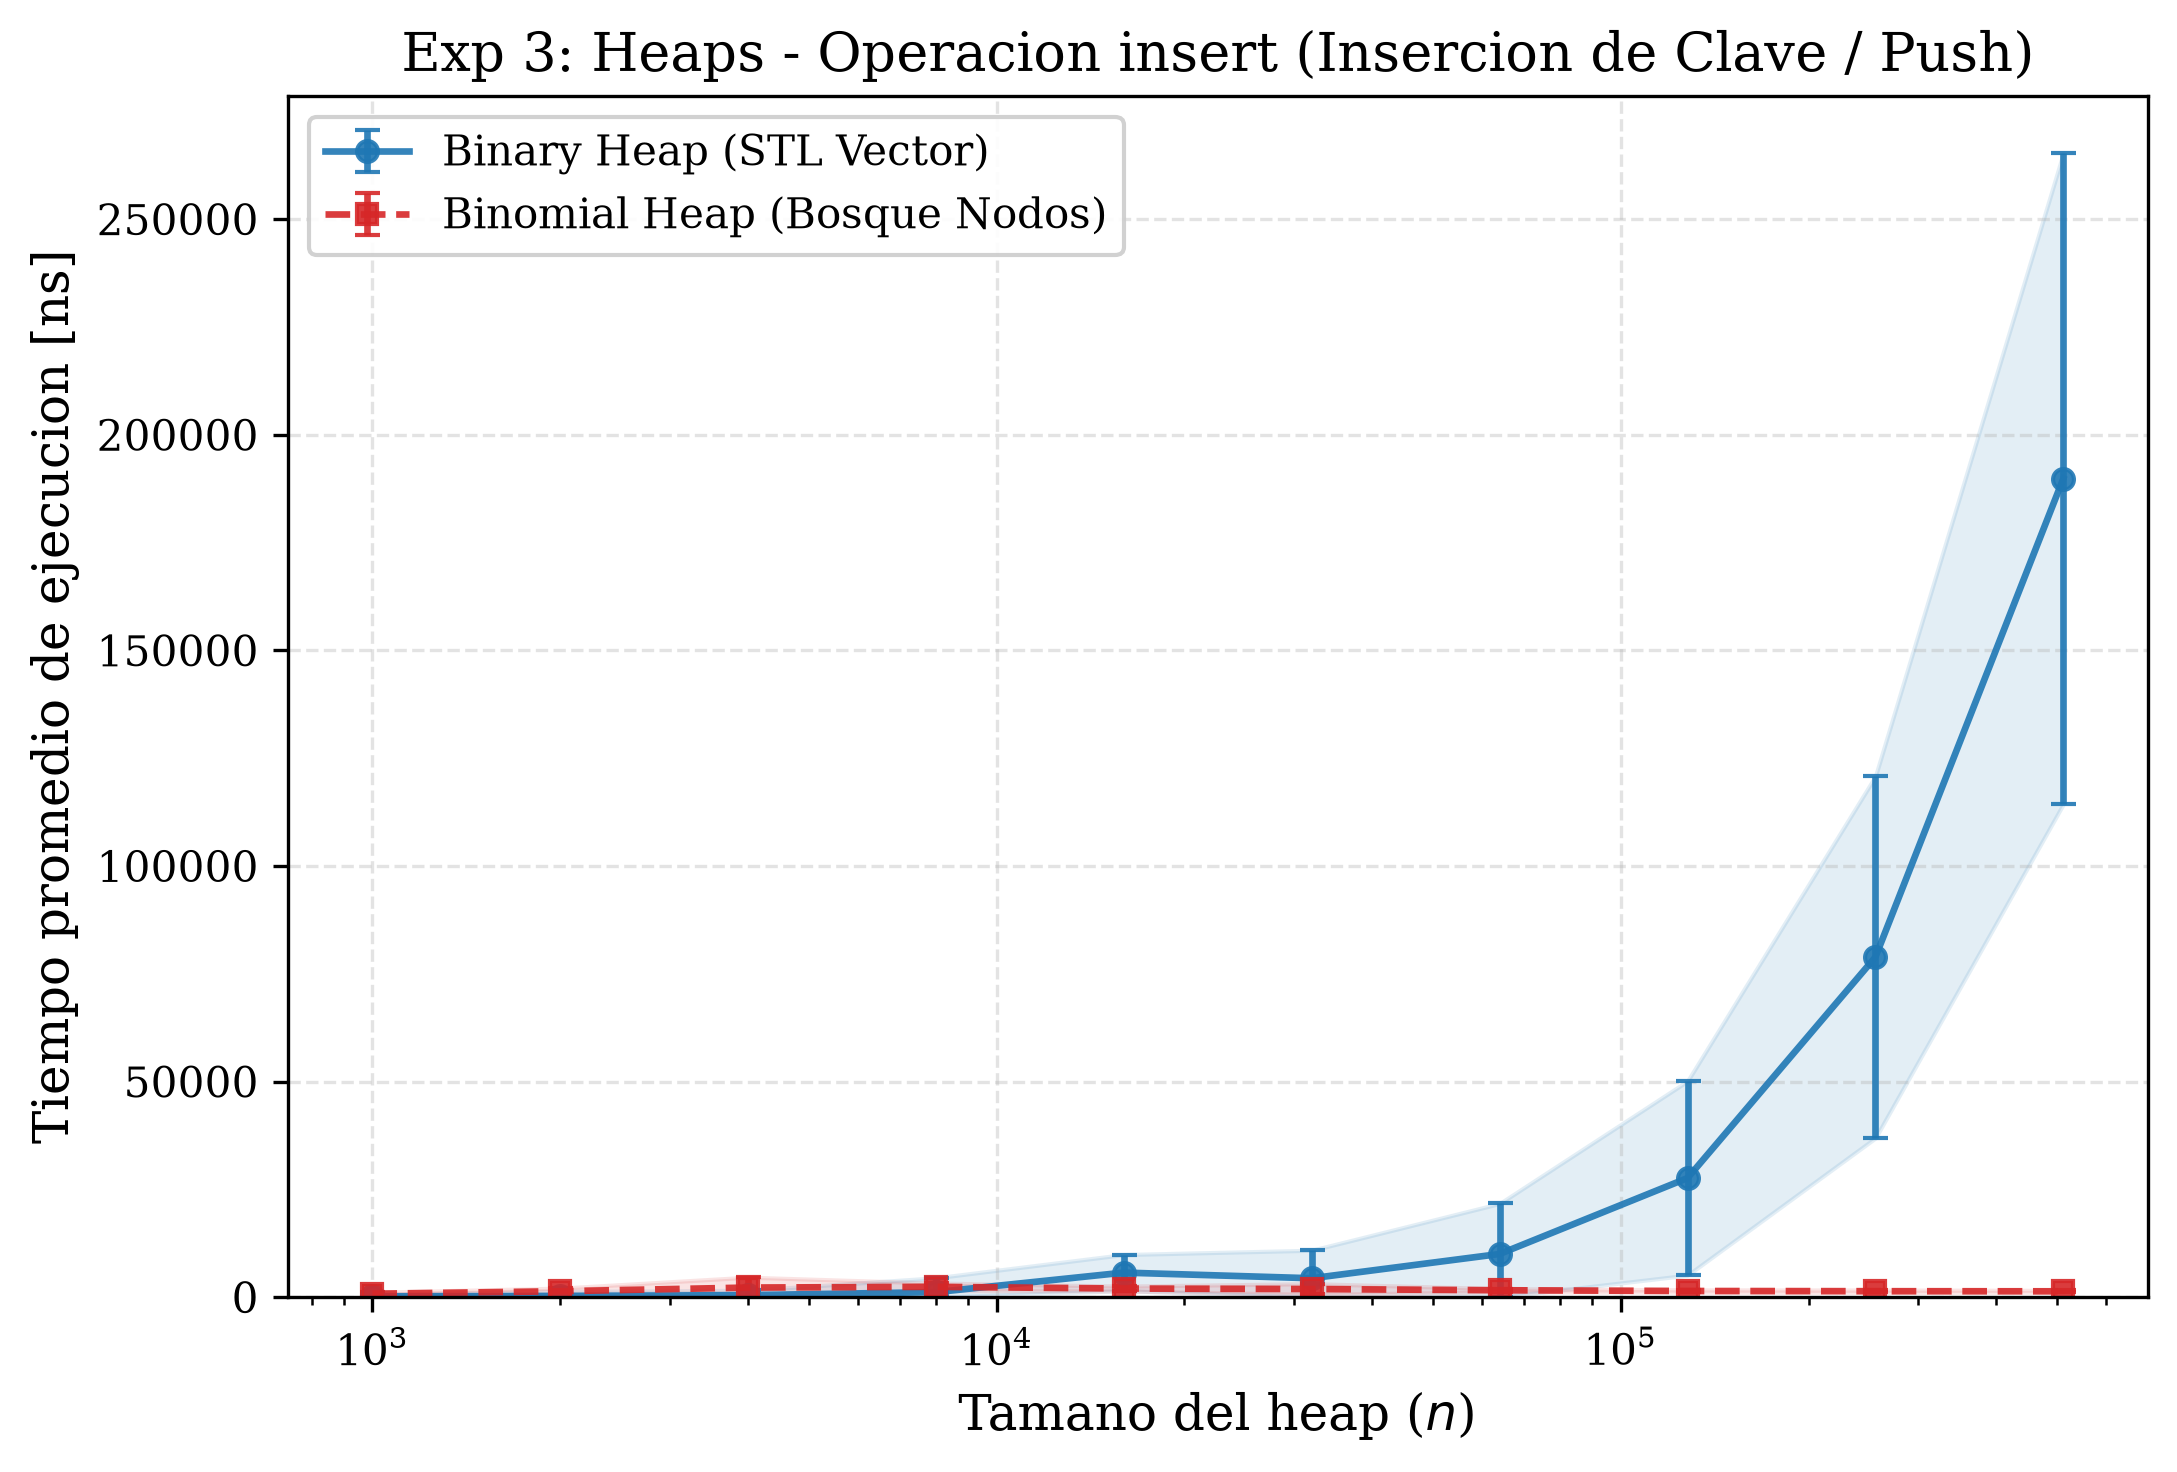
\includegraphics[width=\textwidth]{../plots/Experimento_3_Heaps/fig_heaps_insert.png}
        \caption{\texttt{insert}}
        \label{fig:heap_insert}
    \end{subfigure}
    \hfill
    \begin{subfigure}[b]{0.48\textwidth}
        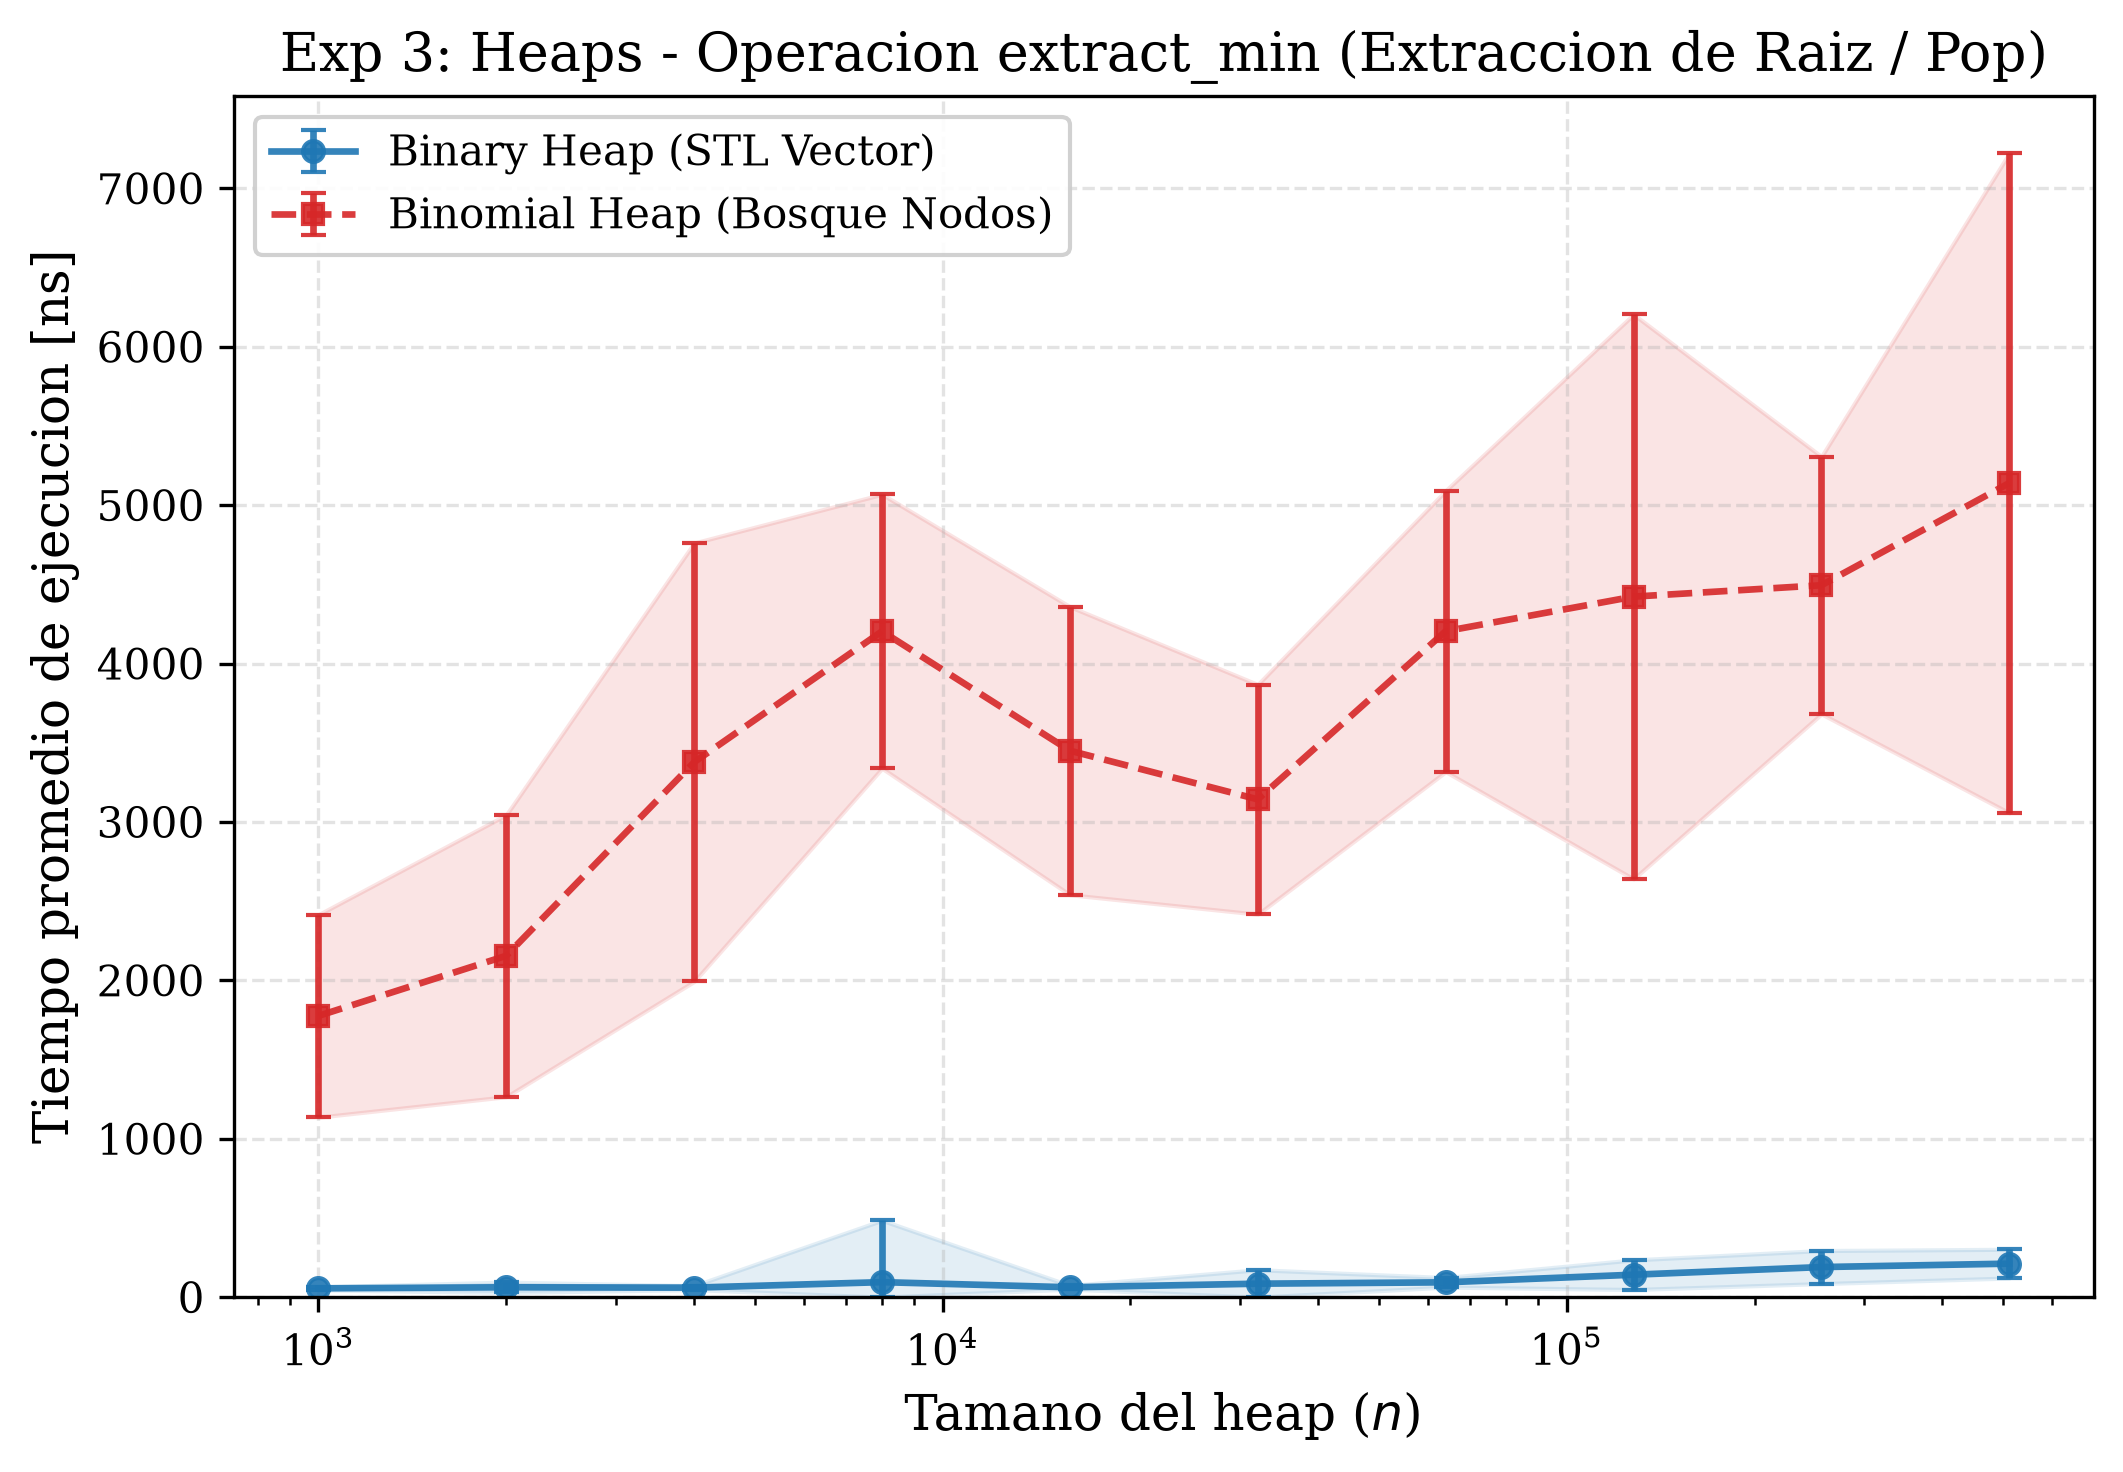
\includegraphics[width=\textwidth]{../plots/Experimento_3_Heaps/fig_heaps_extract_min.png}
        \caption{\texttt{extract\_min}}
        \label{fig:heap_extract}
    \end{subfigure}
    \vskip\baselineskip
    \begin{subfigure}[b]{0.48\textwidth}
        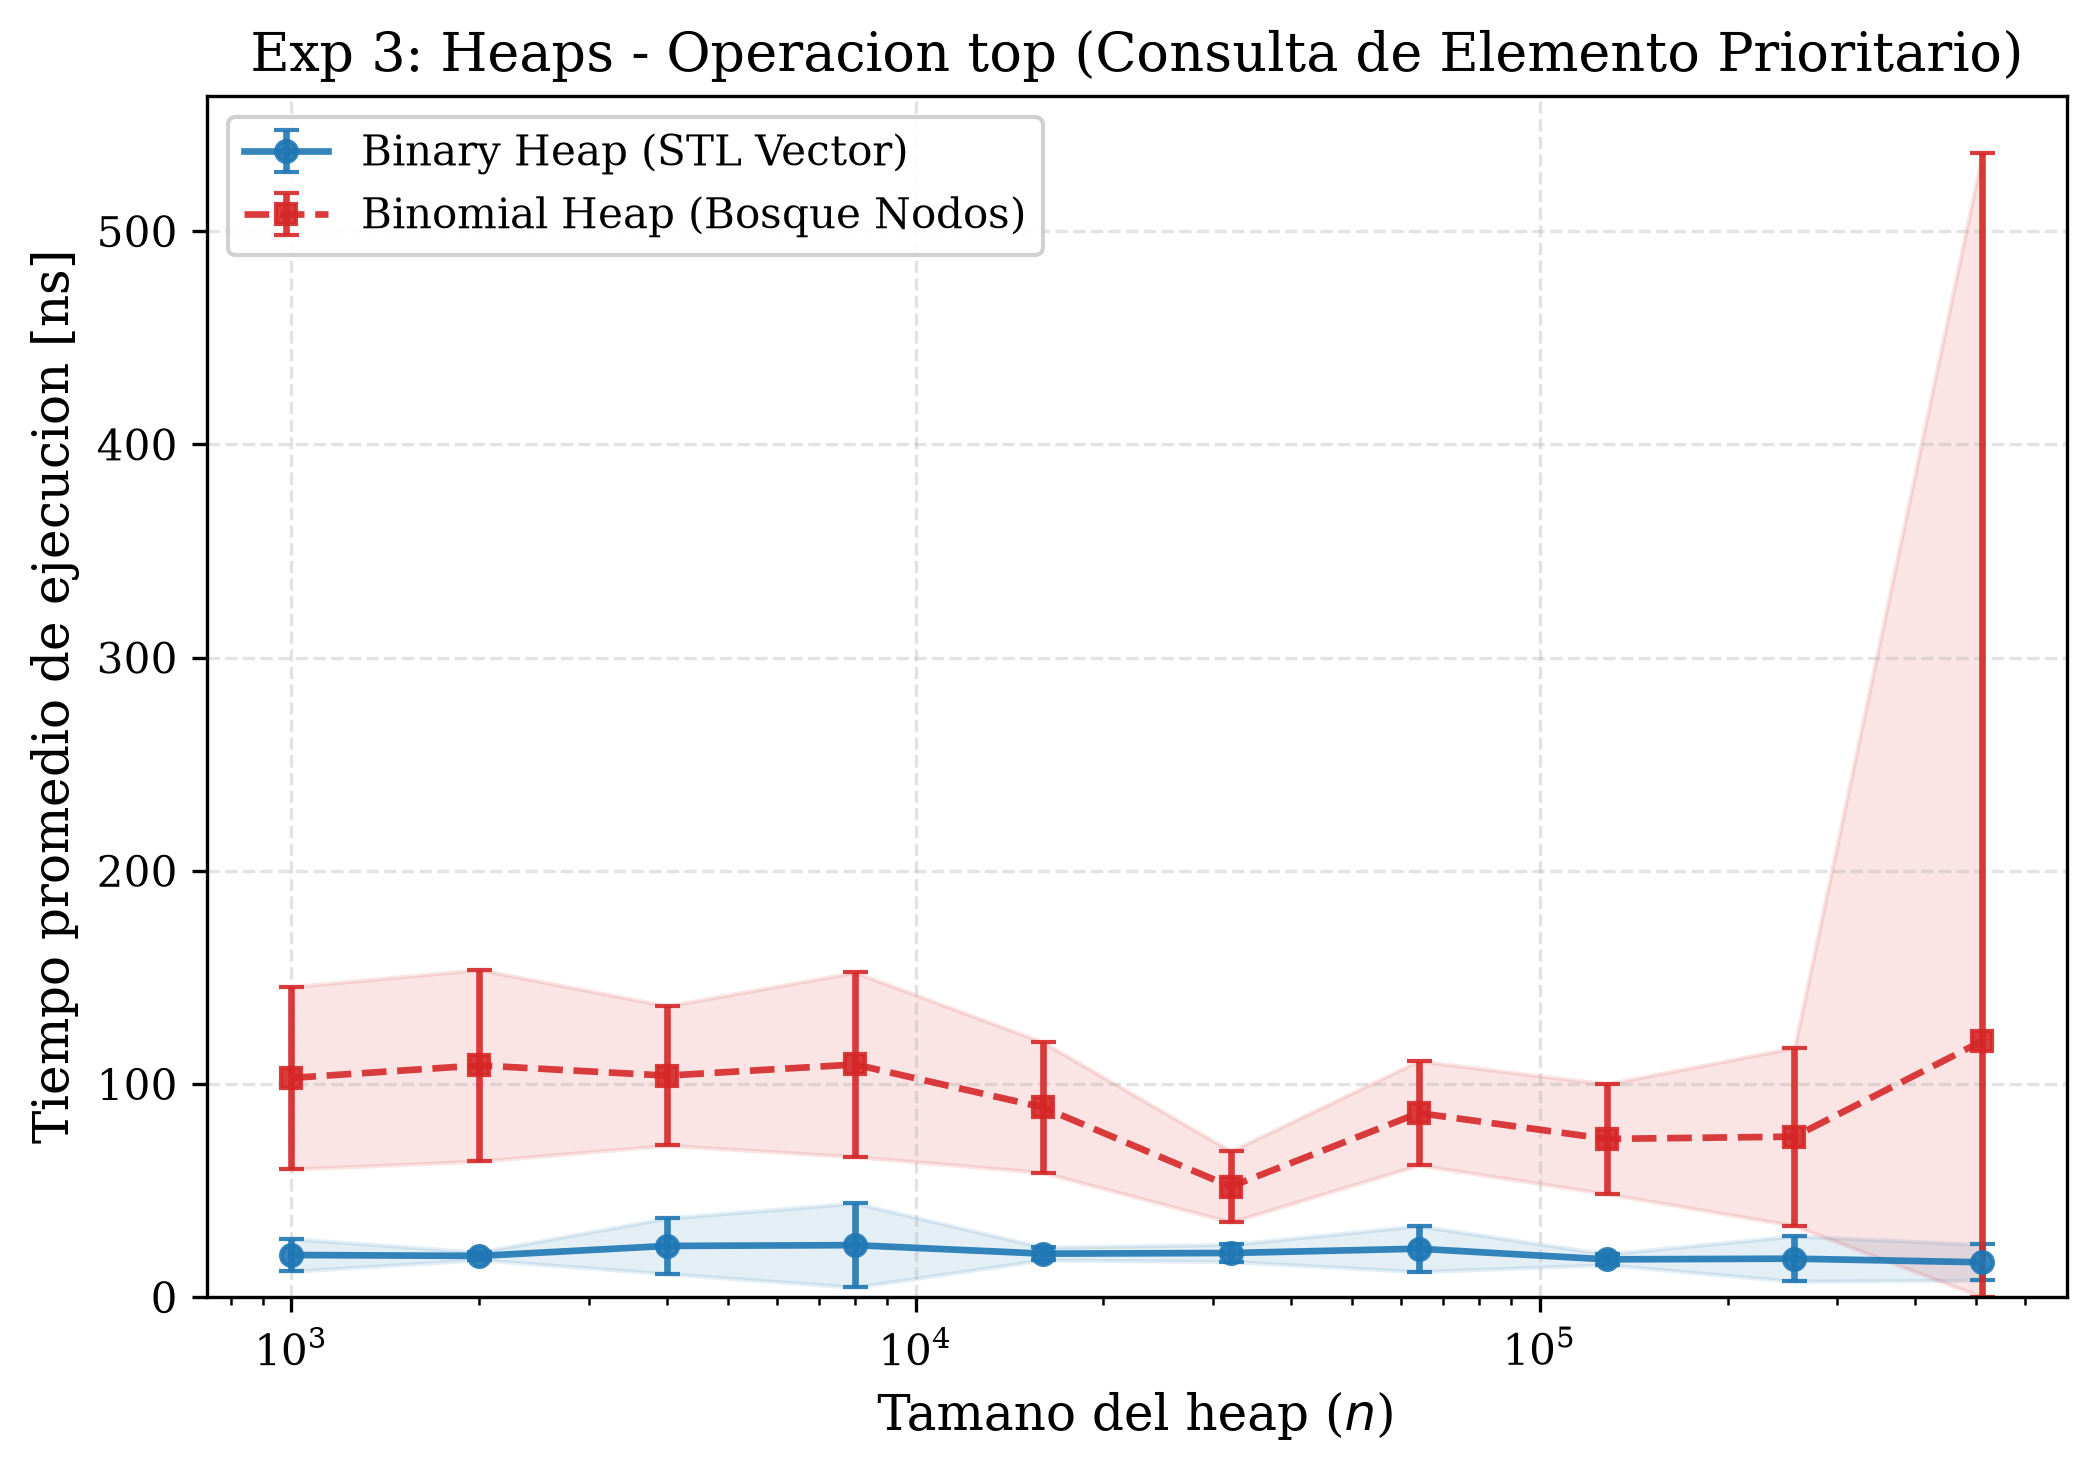
\includegraphics[width=\textwidth]{../plots/Experimento_3_Heaps/fig_heaps_top.png}
        \caption{\texttt{top}}
        \label{fig:heap_top}
    \end{subfigure}
    \caption{Experimento 3: Operaciones elementales de inserción, extracción y consulta.}
    \label{fig:exp3_heaps_elem}
\end{figure}

\paragraph{Observaciones.}
\begin{itemize}
    \item \textbf{build\_heap (Fig.~\ref{fig:heap_build}):} Ambas exhiben tendencia creciente. El Binary Heap registra tiempos notablemente inferiores ($3.63\text{ ms}$ en $n = 512\,000$) frente al Binomial Heap ($358.7\text{ ms}$), una diferencia de $\approx 99\times$.
    \item \textbf{top (Fig.~\ref{fig:heap_top}):} Ambas operan en tiempos constantes del orden de nanosegundos, con el Binary Heap registrando latencias menores.
    \item \textbf{insert y extract\_min (Figs.~\ref{fig:heap_insert} y~\ref{fig:heap_extract}):} Ambas escalas son logarítmicas, siendo el Binary Heap sistemáticamente más rápido en todos los tamaños.
    \item \textbf{meld (Fig.~\ref{fig:heap_meld}):} El Binary Heap escala linealmente ($5.99\text{ ms}$ en $n = 512\,000$). El Binomial Heap se mantiene esencialmente constante ($\approx 2.5\text{--}2.9\text{ }\mu\text{s}$), confirmando su cota $\mathcal{O}(\log n)$. La ventaja del Binomial Heap en fusión alcanza un factor de $\approx 2\,270\times$ en $n = 512\,000$.
\end{itemize}

\newpage
\section{Conclusiones}
A partir de los resultados empíricos obtenidos y contrastados con el análisis teórico previo, se concluye lo siguiente:


\begin{enumerate}
    \item \textbf{Comparación cuantitativa en algoritmos de búsqueda:}
    \begin{itemize}
        \item En arreglos de gran tamaño ($n = 8\,192\,000$), la \textbf{Búsqueda Binaria es en promedio $2\,415$ veces más rápida que la Búsqueda Secuencial} ($850.3\text{ ns}$ frente a $2.053\times 10^6\text{ ns}$), validando la reducción de complejidad de $\mathcal{O}(n)$ a $\mathcal{O}(\log n)$.
        \item En el Experimento 1 (claves uniformes en el rango completo), la Búsqueda Binaria supera a la Galopante por un factor aproximado de $1.57\times$ ($850\text{ ns}$ vs $1337\text{ ns}$), producto del costo adicional de la fase exponencial cuando el valor esperado de la posición es central ($\mathbb{E}[k] = n/2$).
    \end{itemize}
    \item \textbf{Comparación cuantitativa y espacial en colas de prioridad:}
    \begin{itemize}
        \item La estructura \textbf{Binary Heap utiliza aproximadamente una sexta parte del espacio en memoria RAM del Binomial Heap} ($\approx 8\text{ bytes}$ frente a $\approx 48\text{--}56\text{ bytes}$ por elemento), debido a que no requiere almacenar punteros explícitos ni metadatos de fragmentación dinámica por cada nodo.
        \item En operaciones unitarias de inserción y extracción, el Binary Heap es hasta un orden de magnitud más rápido que el Binomial Heap debido a la localidad espacial de caché provista por su representación contigua.
    \end{itemize}
    \item \textbf{Criterios de selección bajo condiciones específicas:}
    \begin{itemize}
        \item \textit{Búsqueda en secuencias:} Si se garantiza que la clave objetivo reside predominantemente en las posiciones iniciales de la secuencia ($k \le 2\%$ del total), es preferible utilizar la \textbf{Búsqueda Galopante} sobre la Binaria, alcanzando reducciones de tiempo de hasta $6\times$ en ese régimen. En caso contrario, si las consultas son uniformes o se distribuyen hacia el final del arreglo ($k > 2\%$), es preferible usar la \textbf{Búsqueda Binaria}.
        
        La \textit{Búsqueda Secuencial} no es particularmente recomendable en ningún escenario, al tener un costo lineal $\mathcal{O}(n)$ que la hace ineficiente frente a las alternativas logarítmicas. Sin embargo cabe recalcar que esta sigue ganando en otros entornos, como por ejemplo cuando se trabaja con secuencias no ordenadas, ya que de los algoritmos estudiados es el único que no requiere ordenamiento previo.
        \item \textit{Colas de prioridad:} Si la aplicación realiza la operación de fusión (\texttt{meld}) con alta frecuencia, es imperativo utilizar el \textbf{Binomial Heap} sobre el Binary Heap, ya que garantiza un costo $\mathcal{O}(\log n)$ frente a la reconstrucción completa $\mathcal{O}(n)$ del vector contiguo. En caso contrario (si predominan \texttt{insert}, \texttt{top} y \texttt{extract\_min}), se debe preferir el \textbf{Binary Heap}.
        \item \textit{Restricción de memoria:} Si se requiere operar en sistemas con memoria restrictiva o entornos de alta concurrencia de caché, se debe emplear el \textbf{Binary Heap}. Si la memoria no es un factor limitante y se requiere unir dinámicamente múltiples colas de prioridad concurrentes, se debe adoptar el \textbf{Binomial Heap}.
    \end{itemize}
\end{enumerate}


\newpage
\section{Referencias}

\begingroup
\renewcommand{\section}[2]{}% Suprime titulo duplicado generado internamente por thebibliography
\begin{thebibliography}{9}
\setlength{\itemsep}{2pt}
\setlength{\parskip}{0pt}

\bibitem{jfuentess_edaa}
jfuentess. (s. f.).
\textit{edaa: Repositorio del curso Estructuras de datos y algoritmos
avanzados} [Código fuente].
GitHub.
\url{https://github.com/jfuentess/edaa}

\bibitem{lovera_github}
Lovera, L. (s. f.).
\textit{Herramientas y arneses de experimentación estadística para EDAA} [Código fuente].
GitHub.
\url{https://github.com/leonardlover}

\bibitem{barbay2007}
Barbay, J., López-Ortiz, A., Lu, T., \& Salinger, A. (2007).
\textit{Faster set intersection algorithms for text searching}
(Technical Report CS-2007-13).
University of Waterloo.
\url{https://cs.uwaterloo.ca/research/tr/2007/CS-2007-13.pdf}

\bibitem{bentley1976}
Bentley, J. L., \& Yao, A. C.-C. (1976).
An almost optimal algorithm for unbounded searching.
\textit{Information Processing Letters, 5}(3), 82--87.
\url{https://doi.org/10.1016/0020-0190(76)90071-5}

\bibitem{demaine2020}
Demaine, E., Ku, J., \& Solomon, J. (2020).
\textit{Lecture 8: Binary heaps}
[Notas de clase del curso 6.006 Introduction to Algorithms].
Massachusetts Institute of Technology, MIT OpenCourseWare.
\url{https://ocw.mit.edu/courses/6-006-introduction-to-algorithms-spring-2020/resources/mit6_006s20_lec8/}

\bibitem{sedgewick_priority_queues}
Sedgewick, R., \& Wayne, K. (s. f.).
\textit{2.4 Priority queues}.
Algorithms, 4th Edition.
\url{https://algs4.cs.princeton.edu/24pq/}

\bibitem{nist_binary_heap}
National Institute of Standards and Technology. (s. f.).
Binary heap.
En \textit{Dictionary of Algorithms and Data Structures}.
\url{https://xlinux.nist.gov/dads/HTML/binaryheap.html}

\bibitem{cpp_heap_operations}
ISO/IEC JTC1/SC22/WG21. (s. f.).
Heap operations [alg.heap.operations].
En \textit{Working draft, standard for programming language C++}.
\url{https://eel.is/c++draft/alg.heap.operations}

\bibitem{cpp_vector_modifiers}
ISO/IEC JTC1/SC22/WG21. (s. f.).
Modifiers [vector.modifiers].
En \textit{Working draft, standard for programming language C++}.
\url{https://eel.is/c++draft/vector.modifiers}

\end{thebibliography}
\endgroup

\subsection{Usos Específicos}
Las implementaciones de referencia y las rutinas de medición de tiempo se tomaron del repositorio del curso \cite{jfuentess_edaa} y de las herramientas del ayudante Leonardo Lovera (\url{https://github.com/leonardlover}) \cite{lovera_github}.

El código fuente desarrollado, los scripts de automatización del banco de pruebas y los datasets generados para este boletín se encuentran alojados en el repositorio de reproducibilidad del proyecto: \url{https://github.com/StackDs/EDAA-Experiments}.

La descripción de la búsqueda galopante se fundamenta en
los trabajos de Bentley y Yao y de Barbay et al.
\cite{bentley1976,barbay2007}.

El análisis de los heaps binarios se apoya en las notas del MIT,
el material de Sedgewick y Wayne y el diccionario del NIST
\cite{demaine2020,sedgewick_priority_queues,nist_binary_heap}.

Las garantías de complejidad de las operaciones de biblioteca
se consultaron en el borrador público del estándar de C++
\cite{cpp_heap_operations,cpp_vector_modifiers}.

\subsection{Declaración De Uso De IA Generativa}
Durante la elaboración de este informe se utilizó ChatGPT, de OpenAI,
como herramienta de apoyo para revisar la redacción académica,
discutir el análisis de complejidad de los algoritmos y contrastar
dicho análisis con las implementaciones estudiadas.
De igual forma se utilizó Google Gemini para estructurar el repositorio con el código fuente y para mejorar los experimentos en términos de optimización.
La responsabilidad por el contenido final, la interpretación de
los resultados y la exactitud de las referencias corresponde
al autor del informe.



\end{document}
